% UCL Thesis LaTeX Template
%  (c) Ian Kirker, 2014
% 
% This is a template/skeleton for PhD/MPhil/MRes theses.
%
% It uses a rather split-up file structure because this tends to
%  work well for large, complex documents.
% We suggest using one file per chapter, but you may wish to use more
%  or fewer separate files than that.
% We've also separated out various bits of configuration into their
%  own files, to keep everything neat.
% Note that the \input command just streams in whatever file you give
%  it, while the \include command adds a page break, and does some
%  extra organisation to make compilation faster. Note that you can't
%  use \include inside an \include-d file.
% We suggest using \input for settings and configuration files that
%  you always want to use, and \include for each section of content.
% If you do that, it also means you can use the \includeonly statement
%  to only compile up the section you're currently interested in.
% You might also want to put figures into their own files to be \input.

% For more information on \input and \include, see:
%  http://tex.stackexchange.com/questions/246/when-should-i-use-input-vs-include


% Formatting rules for theses are here: 
%  http://www.ucl.ac.uk/current-students/research_degrees/thesis_formatting
% Binding and submitting guidelines are here:
%  http://www.ucl.ac.uk/current-students/research_degrees/thesis_binding_submission

% This package goes first and foremost, because it checks all 
%  your syntax for mistakes and some old-fashioned LaTeX commands.
% Note that normally you should load your documentclass before 
%  packages, because some packages change behaviour based on
%  your document settings.
% Also, for those confused by the RequirePackage here vs usepackage
%  elsewhere, usepackage cannot be used before the documentclass
%  command, while RequirePackage can. That's the only functional
%  difference as far as I'm aware.
\RequirePackage[l2tabu, orthodox]{nag}


% ------ Main document class specification ------
% The draft option here prevents images being inserted,
%  and adds chunky black bars to boxes that are exceeding 
%  the page width (to show that they are).
% The oneside option can optionally be replaced by twoside if
%  you intend to print double-sided. Note that this is
%  *specifically permitted* by the UCL thesis formatting
%  guidelines.
%
% Valid options in terms of type are:
%  phd
%  mres
%  mphil
%\documentclass[12pt,phd,draft,a4paper,oneside]{thesis}

\documentclass[12pt,phd,a4paper,oneside]{thesis}

\DeclareMathAlphabet{\mathcal}{OMS}{cmsy}{m}{n} % reset mathcal to non fugly font
\newcommand{\dt}{\mathrm{d}t}
\usepackage{epigraph} %quotes
\usepackage{bm} %bold greek

% Package configuration:
%  LaTeX uses "packages" to add extra commands and features.
%  There are quite a few useful ones, so we've put them in a 
%   separate file.
\input{MainPackages}

% Sets up links within your document, for e.g. contents page entries
%  and references, and also PDF metadata.
% You should edit this!
\usepackage{bibentry}
\makeatletter\let\saved@bibitem\@bibitem\makeatother

\usepackage[pdftex,hidelinks,colorlinks=true,allcolors=black,citecolor=blue]{hyperref}
\makeatletter\let\@bibitem\saved@bibitem\makeatother
\makeatletter
\AtBeginDocument{
    \hypersetup{
        pdfsubject={Biophysics},
        pdfkeywords={inference,bifurcations},
        pdfauthor={Grisha Szep},
        pdftitle={Inferring bifurcations between phenotypes},
    }
}
\makeatother

% And then some settings in separate files.
\input{FloatSettings} % For things like figures and tables
\input{BibSettings}   % For bibliographies

%-----------------------------
%
%   SARS-CoV-2 commands start
%
%-----------------------------
\newcommand{\dihone}{$\mathrm{\xi}_{1}$~}
\newcommand{\dihtwo}{$\mathrm{\xi}^{\mathrm{backbone}}_{2}$~}

\usepackage{tikz} % for inset
   \usetikzlibrary{positioning,spy}

\newcommand{\subfigimg}[3][,]{%
  \setbox1=\hbox{\includegraphics[#1]{#3}}% Store image in box
  \leavevmode\rlap{\usebox1}% Print image
  \rlap{\hspace*{10pt}\raisebox{\dimexpr\ht1-2\baselineskip}{#2}}% Print label
  \phantom{\usebox1}% Insert appropriate spcing
}
%-----------------------------
%
%   SARS-CoV-2 commands end
%
%-----------------------------

%-----------------------------
%
% Protein corona commands start
%
%-----------------------------
\newcommand{\sodium}{Na$^{+}$\,}
\newcommand{\chlorine}{Cl$^{-}$\,}

\newcommand{\vdw}{$\Delta E_{vdW}$}
\newcommand{\elec}{$\Delta E_{elec}$}
\newcommand{\polar}{$\Delta G_{polar}$}
\newcommand{\apolar}{$\Delta G_{apolar}$}
\newcommand{\binding}{$\Delta G_{binding}$}

\newcommand{\code}[1]{\texttt{#1}} %code inline

%\usepackage{amsfonts} % pretty tables
\usepackage{booktabs} % pretty tables
%\usepackage{ulem} % \sout{}
%\usepackage{gensymb} % \degree

\usepackage{siunitx}
\sisetup{
  input-ignore={,},
  input-decimal-markers={.},
  group-separator={,},
  group-minimum-digits=4,
}

%-----------------------------
%
% Protein corona commands end
%
%-----------------------------


%-----------------------------
% misc. packages 
%-----------------------------
\usepackage{notoccite}% PREVENTS CITES IN CAPTIONS FROM MISNUMBERING YOUR REFERENCES 
%-----------------------------
% 
%-----------------------------

% These control how many number sections your subsections will take
%    e.g. Section 2.3.1.5.6.3
%  and how many of those will get put into the contents pages.
\setcounter{secnumdepth}{3}
\setcounter{tocdepth}{3}

\usepackage{pdfpages}
\setboolean{@twoside}{false}
\DeclareMathOperator*{\argmax}{arg\,max}
\DeclareMathOperator*{\argmin}{arg\,min}
\begin{document}
\raggedbottom % stops huge gaps between paragraphs
\nobibliography*
% ^-- This is a dumb trick that works with the bibentry package to let
%  you put bibliography entries whereever you like.
% I used this to put references to papers a chapter's work was 
%  published in at the end of that chapter.
% For more information, see: http://stefaanlippens.net/bibentry

% If you haven't finished making your full BibTex file yet, you
%  might find this useful -- it'll just replace all your
%  citations with little superscript notes.
% Uncomment to use.
%\renewcommand{\cite}[1]{\emph{\textsuperscript{[#1]}}}

% At last, content! Remember filenames are case-sensitive and 
%  *must not* include spaces.
\title{Inferring bifurcations\\between phenotypes}
\author{Grisha Szep}

\department{Randall Division of Cell \& Molecular Biophysics}
\sponsor{Microsoft Research Cambridge}

\date{October 29, 2021}
\maketitle
% \makedeclaration

\begin{abstract} % 300 word limit

    The gene-expression history of an organism and its environment determine the organism's phenotype. The phenotype is an inherently qualitative state, deduced by relative biochemical concentration measurements collected by methods such as flow cytometry or fluorescence microscopy. The biochemical threshold concentrations that distinguish different phenotypes can be modelled by applying bifurcation analysis to differential equation models and the search for these boundaries in experimental data can be done using dimensionality reduction and clustering techniques. This establishes a relationship between bifurcations, phenotypes and machine learning techniques that are the subject of this thesis.

    % The first chapter presents an interactive tool for exploring phenotypes in flow cytometry data. In particular we explore a multi-tissue, high-dimensional, immune cell dataset. The tool bridges machine learning methods and the popular FlowJo, used to annotate cells with gating strategies. An assortment of dimensionality reduction techniques are applied to create two dimensional embeddings and confusion matrices are used to quantify annotation agreement between immunologists. By leveraging the geospatial mapping library OpenLayers to render, annotate and analyze cells, immunologists can now efficiently navigate the phenotype space of Human Cell Atlas datasets.
    
    % The next chapter focuses on a model-driven approach for exploring and designing phenotypes, where we demonstrate how model-guided design of synthetic E. Coli can elucidate pattern formation mechanisms in multicellular development. We infer the parameters of a biochemically motivated system of differential equations against time course fluorescence data acquired from plate reader experiments. Our design goals however were not in the temporal domain, rather we wanted to control the shape and size of a cusp bifurcation in the space of experimentally controlled input concentrations.
    
    % To address these limitations, I define a differentiable semi-supervised cost function that uses bifurcation locations as targets. Bifurcations are encouraged by an unsupervised term that extremises the curvature of the determinant of the Jacobian. By exploring the cost landscape for minimal models that span the space of saddle-nodes and pitchforks, I show that the parameter space basins define regions of qualitatively equivalent differential equations. The differentiability of the cost function enables efficient optimisation using libraries such as Flux.jl that leverage automatic differentiation. The impact of this work would enable experimentalists to efficiently navigate design spaces of differential equation models.
    
\end{abstract}
\newpage
\clearpage
\begin{center}
    \thispagestyle{empty}
    \vspace*{\fill}
    \epigraph{
        Blank pages are the worst.\\
        They impose a glaring responsibility onto someone to fill it with meaningful content.\\
        Much like other starting points:
        a new job, a marble stone, empty land, all future that tower over you, forcing the person facing it to ask:\\
        "do I really want to do this?"\\
        Blank pages are the worst.\\
        They reflect a glaring light upon you, reflecting the messages that would otherwise happinly bounce around in the ether, along with memories, desires, unfinished projects, and other concofonous bullshit in your head.\\
        A whole page!\\
        Rejoice at the etchings of achievement. You've started now so don't give up, or stop, you'll look stupid. Now make sure you go back and edit the previous page so that other will not know how stupid you are.\\
        Edit it, edit it,\\
        edit it into oblivion untill you can't recognise whether you are editing the page or yourself.}{}
    \vspace*{\fill}
\end{center}
\clearpage

\begin{acknowledgements}
    The past four years of my life have been full of excitement, creativity and exploration, none of which would have been possible without the support of Attila and Neil. Their mentorship and guidance has been a shining example of leadership and whose qualities I will take with me into future roles. I would like to thank my colleagues and friends at Microsoft Research, whose diverse projects in biotechnology captured my imagination.

    I would like to acknowledge Valerie Coppard, who was an absolute pleasure to work with and introduced me to Joanne Jones' lab at Cambridge University, catalysing the \emph{FlowAtlas.jl} project. Her enthusiasm...

    I would like to thank Matilda Peruzzo and Silvia Cabaliero During the pandemic. I would like to thank Mohammed Ali

    I am thankful to my friends at Burnt Umber who run a cozy and welcoming cafe in Hackney Wick, where I wrote a large chunk of my thesis, felt supported and cared for during difficult times. Disree Shaw my therapist. Fraser...

    I would like to thank family and dad
\end{acknowledgements}

%%%%%%%%%%%%%%%%%%%%%%%%%%%%%%%%%%%%%%%%
%%%%%%%%%%%%%%%%%%%%%%%%%%%%%%%%%%%%%%%%
%%%%%%%%%%%%%%%%%%%%%%%%%%%%%%%%%%%%%%%%
%%%%%%%%%%%%%%%%%%%%%%%%%%%%%%%%%%%%%%%%
%%%%%%%%%%%%%%%%%%%%%%%%%%%%%%%%%%%%%%%%

\setcounter{tocdepth}{2} 
% Setting this higher means you get contents entries for
%  more minor section headers.

\tableofcontents
\listoffigures
\chapter{Introduction}
\label{Motivation}
%
\epigraph{\textit{I wish to God these calculations had been executed by steam.}}{Charles Babbage}
The advent of the modern digital computer, as formalised by Alan Turing,\cite{Turing1937} ignited the field of computational physics, aided by preexisting theoretical formulations of algorithms. Starting from the first experiments with Monte Carlo (MC) simulations in the 1930s by Fermi and the formulation of the Markov-Chain Monte Carlo (MCMC) technique by Ulam in the 1940s, von Neumann programmed the 18,000 vacuum-tube Electronic Numerical Integrator and Computer (ENIAC) computer to investigate neutron diffusion in fissionable materials.\cite{metropolis1987beginning} This success paved the way for the integration of Newton's equations of motion to compute the time evolution of a many-body system.\\

\section{Current state-of-the-art in biomolecular simulations}
\label{sec:sota_bio_sims}
\subsection{Groundbreaking simulations}

\subsection{Bespoke forcefield parametrisation}
\label{sec:ff_devel}

\subsubsection{OpenFF initiative}

\subsubsection{Gaussian process regression}

\subsubsection{Neural network forcefields}

\subsubsection{QUBE forcefield}

\subsubsection{Outlook}

%%%%%%%%%%%%%%%%%%%%%%%%
%     Architectures
%%%%%%%%%%%%%%%%%%%%%%%%
\subsection{State of the art architecture}

\subsubsection{GPU acceleration}

\subsubsection{ASIC}

\subsubsection{FPGA}

%%%%%%%%%%%%%%%%%%%%%%%%
%    Finally, make 
%     your case 
%%%%%%%%%%%%%%%%%%%%%%%% 
\section{Motivation}

\chapter{Theoretical Background}
\label{Introduction}

\epigraph{``\textit{You must understand, young Hobbit, it takes a long time to say anything in Old Entish. And we never say anything unless it is worth taking a long time to say.}"}{J.R.R. Tolkien}

\section{Molecular dynamics}\label{chapter:MD}

\subsection{Numerical integrators} \label{sec:integrators}
%
%\epigraph{``To do the same thing over and over again is not only boredom: it is to be controlled by rather than to control what you do."}{Heraclitus}
%

\subsection{Initial configuration} 

\subsection{Periodic boundary conditions}

\subsection{Equilibration} \label{sec:equilibration}

\subsubsection{Energy minimisation}

\subsubsection{Particle velocities}

\subsection{Thermostats}
%
%\epigraph{``The worst thing you can do about a situation is nothing."}{Ice Cube}

\subsection{Parallelisation}

\subsubsection{Domain decomposition}

\subsubsection{Particle-mesh-Ewald summation} \label{sec:pme}

% ---------------------
%
%       DFT INTRO
%
% ---------------------
\section{Density Functional Theory} \label{chapter:onetep}

\subsection{Hohenberg-Kohn Theorems}

\subsection{Kohn-Sham equations}
\chapter{Accurate large scale modelling of Graphene Oxide}
\label{GO}
%\epigraph{``No person will deny that the highest degree of attainable accuracy is an object to be desired, and it is generally found that the last advances towards precision require a greater devotion of time, labour, and expense, than those which precede them."}{Charles Babbage}
\vspace{-9mm}
The development of accurate structures and forcefield parameters for exotic materials are paramount to the transferability of molecular dynamics investigations. Using preexisting work that posits the semi-ordered structure of graphene-oxide (GO), implemented using software developed to create semi-ordered rectangular graphene oxide sheets, we develop a bespoke forcefield using density functional theory calculations. We compare the performance of both generalised and bespoke forcefields on the behaviour of GO in solution with respect to experiments. We discover that observables diverge between generalised and bespoke forcefields in interfacial water dynamics and ion adsorption. This work provides an insight to the importance of bespoke forcefield design for combining both accuracy and scale in modelling nanomaterials at the interface. \edit{The bespoke forcefield shows strong agreement with AIMD simulations for the interfacial water dynamics and ion adsorption; we conclude that this results in the forcefield having an accuracy near that of AIMD.} \edit{Contributions for this work are as follows: \textbf{Mohamed Ali al-Badri} and \textbf{Christian D. Lorenz} conceived and planned the research. \textbf{Mohamed Ali al-Badri} and \textbf{Robert C. Sinclair} developed the nanomaterial structure software. \textbf{Mohamed Ali al-Badri} performed the calculations. \textbf{Mohamed Ali al-Badri, Paul Smith} and \textbf{Christian D. Lorenz} analysed the data and \textbf{Mohamed Ali al-Badri} prepared the final manuscript.}

%Contributions for this work are as follows: \textbf{Mohamed Ali al-Badri}: Conceptualisation, Methodology, Software, Validation, Formal analysis, Investigation, Writing - original draft, Visualisation. \textbf{Paul Smith}: Methodology, Software \edit{development for analysis scripts}, Validation, Formal analysis, Visualisation. \textbf{Robert C. Sinclair}: Methodology, Software \edit{development for creating the nanomaterial structures}. 

%addtotoc Adds an entry to the table of contents. This option requires five
%arguments, separated by commas:
%addtotoc={⟨page number ⟩,⟨section ⟩,⟨level ⟩,⟨heading ⟩,⟨label ⟩}
%⟨page number ⟩: Page number of the inserted page.
%6
%⟨section⟩: LATEX sectioning name – e.g., section, subsection, . . .
%⟨level⟩: Number, denoting depth of section – e.g., 1 for section level, 2 for
%subsection level, . . .
%⟨heading⟩: Title inserted in the table of contents.
%⟨label⟩: Name of the label. This label can be referred to with \ref and
%\pageref.


\includepdf[pages=-, offset=75 -75,addtotoc={
     1,section,1,Introduction,p1,
     2,section,1,Results,p2,
     2,subsection,2,Forcefield parameters,p2,
    %2,subsection,3,Structural fluctuations,p2,
     2,subsection,2,Water structure,p2,
    % 3,subsection,3,Interfacial water,p3,
    % 5,subsection,3,Ion adsorption,p5,
     7,section,1,Conclusions,p7,
     9,section,1,Methods,p9,
     9,subsection,2,Geometry,p9,
     9,subsection,2,Molecular Dynamics,p9,
     9,subsection,2,Density Functional Theory,p9},
     addtolist={
     3, figure,{The semi-ordered 979 atom GO sheet structure, showing regions of oxidised and unoxidised domains. Inset images highlight the structures and naming convention of aromatic carbon and alcohol, epoxy, phenol and carboxyl functional group atoms.},b,
     3, figure, {The distribution of DDEC (A) partial charge, (B) Lennard Jones $\epsilon$ and (C) Lennard Jones $\sigma$ non-bonded forcefield parameters for the component atom types of the GO sheet.OPLS parameters are presented as dashed lines.},c,
     3, figure, {The lateral illustration of OPLS and DDEC partial charges of the graphene-oxide sheet.},c,
     4,figure, {The structural deformation of the GO sheet in solution, measured by the distance from the mean in the orthogonal plane for the duration of the MD simulation for DDEC(left) and OPLS (right) forcefields.},d,
     4, table, {Mean number of intramolecular and intermolecular GO hydrogen bonds according to atom type for DDEC and OPLS GO, where the highest numbers of hydrogen bonds are highlighted. Intramolecular hydrogen bonds are normalised by the number of donor atoms. Water-GO hydrogen bonds are normalised by the number of GO atoms. Columns and rows denote accepting and donating species, respectively. Zero hydrogen bonds are denoted as dashes.}, e,
     5, figure, {The radial distribution functions of water oxygen atoms to the component GO (A) oxygen and (B) carbon atom types, according to both DDEC and OPLS forcefields and their respective hydration numbers for (C) oxygen and (D) carbon atom types.}, f,
     5, figure, {The correlation of GO atom coordination number by (A) water molecules, (B) Na$^{+}$ and (C) Cl$^{-}$ ions between the OPLS and DDEC forcefields, labeled by atom type. }, g,
     6,figure, {Intrinsic structure of the GO-water interface for both OPLS and DDEC forcefields, as indicated by (A) the intrinsic density profile, normalised to its bulk value, (B) the number of water-water hydrogen bonds ($N_{HB}$), (C) the density-weighted profile of dipole orientation ($\tilde{P}$) and (D) the density-weighted intrinsic profile of the second moment of dipole orientation ($\tilde{T}$).}, h,
     7,figure, {The joint probability density $\rho(z, \theta_{\mu})$ of the water dipole angle $\theta_{\mu}$ as a function of $z$ from the intrinsic surface of the GO sheet in solution, for both DDEC and OPLS forcefields. The difference plot shows $\rho^{\rm{DDEC}}(z, \theta_{\mu})\,-\, \rho^{\rm{OPLS}}(z, \theta_{\mu})$}, i,
     7, figure, {The radial distribution functions of sodium ions to the component GO (A) oxygen and (B) carbon atom types, according to both DDEC and OPLS forcefields and their respective mean coordination numbers for (C) oxygen and (D) carbon atom types. Error bars indicate the standard error of the mean.}, j,
     8, figure, {The radial distribution functions of chlorine ions to the component GO (A) oxygen and (B) carbon atom types, according to both DDEC and OPLS forcefields and their respective mean coordination numbers for (C) oxygen and (D) carbon atom types. Error bars indicate the standard error of the mean.}, k,
     8, table, {Adsorption half-life (ps) of ion atoms around each GO carbon type}, l,
     8, table, {Adsorption half-life (ps) of ion atoms around each GO oxygen type},m}
    ]{PDF_PAPERS/carbon_paper.pdf}      
%    ]{PDF_PAPERS/carbon_paper_fixed.pdf}      

\section*{Erratum}

    \edit{Due to an error in the plotting script, Fig.~(3.2) has been modified to accurately illustrate the distribution of OPLS and DDEC forcefield parameters. This error has no impact on the discussion, results nor other plots in the chapter. In Fig.~(\ref{fig:fixed_ddec_params} A,C), the legend colours now correctly reference the respective atom types, unlike Fig.~(3.2). The distance between the Lennard-Jones $\epsilon$ values is correctly plotted in Fig.~(\ref{fig:fixed_ddec_params} B), where previously a distribution was wrongly plotted for the DDEC values.}

\begin{figure}[ht!]
    \centering
    \includegraphics[width=1.0\linewidth]{ddec_params.png}
    \caption{\edit{The distribution of DDEC (A) partial charge, (B) Lennard Jones $\epsilon$ and (C) Lennard Jones $\sigma$ non-bonded forcefield parameters for the component atom types of the GO sheet. OPLS parameters are presented as dashed lines in (A) and (C), the absolute difference between the OPLS (triangle) and DDEC (circle) Lennard Jones $\epsilon$ values (gray: negative, black: positive).}}
    \label{fig:fixed_ddec_params}
\end{figure}

%addtolist={⟨page number ⟩,⟨type ⟩,⟨heading ⟩,⟨label ⟩}
%⟨page number ⟩: Page number of the inserted page.
%⟨type⟩: Name of a floating environment. (figure, table, etc.)
%⟨heading⟩: Title inserted into LoF, LoT, etc.
%⟨label⟩: Name of the label. This label can be referred to with \ref and
%\pageref.

% Actually this is a much better solution! Page command may also automatically number the pages
%\includepdf[
%  pages=1,  offset=75 -75]{PDF_PAPERS/carbon_paper.pdf}
% \addcontentsline{toc}{section}{Introduction}
%\includepdf[
%  pages=2,
%  pagecommand=\phantomsection\addcontentsline{toc}{section}{File 02, Page 2},
%]{file_01.pdf}

%Ignore this: 
%\addcontentsline{toc}{section}{Introduction} %this will need enhanced anchoring in the respective pages
%\addcontentsline{TABLE}{LEVEL}{TITLE}
%TABLE stands for the type of list, where you want to add the item, possible are:
%
%toc: Table of contents
%lof: List of figures
%lot: List of tables
%LEVEL will be the level at which the line will appear in the list. Possible are:
%
%For toc: chapter, section, subsection
%For lof: figure
%For lot: table
%TITLE is your heading.


%\addcontentsline{lof}{figure}{Test caption!}
%\includepdf[pages=-, offset=75 -75]{PDF_PAPERS/carbon_paper.pdf}
% \chapter{Nanomaterial functionalisation modulates hard protein corona formation} \label{ProteinCorona}

%\epigraph{\textit{I Have divers times endeavoured to see and to know, what parts the Blood consists of; and at length I have observ’d, taking some Blood out of my own hand, that it consists of small round globuls driven thorough a Crystalline humidity or water: Yet, whether all Blood be such, I doubt.}}{Antoni Van Leeuwenhoek}

%\begin{center}
%    \textit{The contents of this chapter are under review with Nanoscale Horizons}
%\end{center}

The work in this chapter extends on the accurate modelling of graphene oxide nanomaterials to investigate changes in protein structure upon adsorption on the material. Using molecular dynamics simulations, we study the evolution of protein structure in response to interfacial interactions on the bio-nano interface. To understand the impact of structural changes over simulation times of hundreds of nanoseconds, we require a comprehensive analysis pipeline that investigates these changes from multiple perspectives. Here, we probe the varying adsorption behaviours of apolipoprotein c-III and the effect of functional groups in modulating protein aggregation on the nanomaterial. We use two functionalisations of graphitic materials --- graphene oxide and double-clickable graphene oxide.

\edit{Contributions for this work are as follows: \textbf{Mohamed Ali al-Badri} and \textbf{Christian D. Lorenz} conceived and planned the research. \textbf{Mohamed Ali al-Badri} performed the calculations. \textbf{Mohamed Ali al-Badri, Paul Smith} and \textbf{Christian D. Lorenz} analysed the data and \textbf{Mohamed Ali al-Badri} prepared the final manuscript.}
%Contributions for this work are as follows: \textbf{Mohamed Ali al-Badri}: Conceptualisation, Methodology, Software, Validation, Formal analysis, Investigation, Writing - original draft, Visualisation. \textbf{Paul Smith}: Methodology, Software \edit{development for analysis scripts}, Validation, Formal analysis, Visualisation.
\clearpage

The protein corona is an obstacle to exploiting the exotic properties of nanomaterials in clinical and biotechnology settings, with potential applications in DNA sequencing, point of care testing and drug delivery vehicles. The formation of the protein corona is driven by dynamic atomic scale interactions at the bio-nano interface, which are impenetrable using conventional experimental techniques. Here, we use molecular dynamics simulations to study the effect of graphene-oxide (GO) functionalisation on apolipoprotein-c3 (apo-c3) adsorption. We develop an analysis pipeline, encompassing binding energy calculations to protein structure analyses employing \edit{Uniform Manifold Approximation and Projection for Dimension Reduction (UMAP)} and machine learning clustering. We find that apo-c3 is denatured by adsorption on GO, largely driven by the large energetic contributions of electrostatic interactions such as $\pi$-$\pi$ stacking of aromatic amino acids to pristine graphene regions. The enthalpic contribution of such binding event outweighs the intraprotein bond enthalpy required to maintain the protein tertiary structure. Through denaturing and exposing buried hydrophobic residues, the protein backbone is stabilised by forming $\beta$-bridges, which serve as binding motifs for protein-protein interactions that drive further protein aggregation on the nanomaterial surface. When adsorbing on double-clickable azide- and alkyne-double functionalised graphene oxide (C2GO), apo-c3 largely retains its tertiary structure. Binding with the nanomaterial surface is dominated by weaker van der Waals interactions that are dispersed over the protein surface, where charged protein residues are sterically hindered by azide functional groups. The apo-c3 N-terminus is the binding motif for C2GO adsorption, leaving the  conformation of the C-terminus unchanged, hence conserving the lipid binding function of apo-c3.

\section{Introduction}

Graphene-oxide (GO) is a semi-ordered 2D material that shares many novel mechanical and electronic properties with graphene. It is utilised in applications including ion trapping, desalination, electronics, chemistry and biomedicine.\cite{yuan2017enhanced, zhu2010graphene, chung2013biomedical} GO is a promising platform for \textit{ex} and \textit{in vivo} biological applications --- such as bio-sensing and therapeutics. Its electrochemical properties makes GO an attractive contender for bio-sensing applications such as single nucleotide polymorphism detection in DNA,\cite{bonanni2012inherently} next generation nanopore DNA sequencing \cite{heerema2016graphene} and point of care (PoC) applications for early virus detection using covalently linked immobilised monoclonal antibodies.\cite{afsahi2018novel} Therapeutically, the large surface area to volume ratio of 2D materials results in a large loading capacity for targeting molecules, fluorescent dyes and drug molecules for intravenous administration as well as photothermal therapy for cancer treatment.\cite{robinson2011ultrasmall, liu2013graphene, sun2008nano, zhang2010functional}  \\

Unfortunately the transition from \textit{in vitro} to clinical settings is held back by a chemically driven adsorption of serum proteins --- referred to as a protein corona --- upon their introduction to a biological medium.\cite{casals2010time, ke2017decade} A hard corona (HC) is a tightly bound monolayer of proteins at the nanoparticle interface. Subsequent protein layers adherent to the HC are referred to as the soft corona (SC).\cite{rocker2009quantitative} The character and composition of the HC define the nanomaterial's biological identity and therefore its biological fate, circulation time, cellular uptake and cytotoxicity.\cite{nierenberg2018formation, mei2018protein} HC formation has revealed highly variant protein composition profiles, sensitive not only to inter-species biological media \cite{solorio2017comparison} but also disease-specific influences in human GO coronas.\cite{hajipour2015personalized} Patient-specific or `personalised' protein corona profiles have since been utilised as a diagnostic tool for high-throughput, inexpensive and highly accurate early cancer detection.\cite{papi2019converting} \\

Modulating the HC character to overcome the disadvantages of 2D materials in biological applications through nano-functionalisation remains challenging.\cite{rampado2020recent} Extrapolating the sensitivity of nano-functionalisation to the aforementioned highly variant identity of the corona from experimental studies is incomplete and requires a better understanding of GO-HC interfacial behaviour to atomistic precision. Such an understanding is paramount to designing the next generation of biosensors and nanomedicines.\\

Azide- and alkyne-double functionalised graphene oxide (C2GO) has previously been proposed as a cancer targeting nanovector,\cite{mei2015synthesis} where click reactions conjugate targeting moieties on azide and trimethylsilyl (TMS)-alkyne functional groups.\cite{rubio2015solvent} In vitro, both C2GO and GO show varying HC character when exposed to serum proteins, which subsequently impacts their biological identities.\cite{mei2018protein} An experimental quality-by-design screening platform was used to unpick the HC character and evaluate its relationship with biological fate, cellular uptake and cytotoxicity. Using this, proteins that reduced material dependent toxicities were identified to play a role in diminishing cytotoxicity, including apolipoprotein C-III (apo-c3).\cite{mei2018protein} \\

Protein coronas are known to temporally evolve, leaving the total amount of protein constant but varying their composition according to binding affinity, known as the Vroman effect.\cite{vroman1980interaction} Upon the introduction of a nanomaterial to a biological medium, highly abundant proteins such as albumin, immunoglobulin G and fibrinogen bind to the nanoparticle surface in the early stages of the Vroman effect, followed by their replacement with high binding affinity proteins such as apolipoproteins and coagulation factors in the late stages of the Vroman effect.\cite{foroozandeh2015merging, ehrenberg2009influence, harnisch2000adsorption, goppert2005polysorbate, vroman1980interaction} The Vroman effect has previously been observed in computational and experimental studies of peptide, cellulose and fatty-acid binding on GO.\cite{radic2013competitive} \\

 Previously, MD has been used to study the interactions of GO with peptides to understand conformational transitions of amyloid-beta during adsorption,\cite{baweja_effect_2015} the hydration pattern of an adsorbed toy-model alpha-helix \cite{baweja2013hydration} and verification of enzyme active-site deformation following adsorption. \cite{sun_mechanism_2014} To the best of our knowledge, no MD simulations have so far studied protein adsorption on accurate models of GO, and have instead randomly placed oxidised functional groups on the GO surface. Accurate modelling of GO should reflect the semi-ordered structure of GO; composed of inhomogeneous regions of oxidised and unoxidised domains, where amorphous alcohol and epoxy groups make up the oxidised regions.\cite{sinclair2019modelling} \textit{Ab initio} MD simulations of GO show that semi-ordered models of GO are the most stable structures in vacuum as well as in liquid water.\cite{mouhat2020structure} Furthermore, we have recently shown the importance of accurate functionalisation and accounting for steric strain and edge functional groups in large scale MD simulations of GO, using generalised and bespoke electronic structure MD forcefield design.\cite{al2020accurate} In this work, we use molecular dynamics (MD) simulations to study protein denaturing through adsorption on GO and C2GO, to understand HC conformation-activity relationships through binding free energy, contact map, protein structure and solvent exposure analyses. We apply machine learning dimensionality reduction techniques to decode the spatio-temporal MD data that is hard to interpret into distinct protein secondary structure conformations.
%--------------------------------------
%
%               RESULTS
%
%--------------------------------------
\section{Results}
%
\subsection{Binding on the bio-nano interface}
%
In both GO and C2GO systems, apo-c3 readily adsorbs to the substrate and reaches a stable conformation over the course of the adsorption trajectory. To investigate the binding of apo-c3 to the GO and C2GO interface, we compute contact maps and free energies of binding that underpin the changes in protein structure following adsorption. These analyses probe interfacial dynamics that may play a large role in the formation of a protein corona around a nanomaterial upon its introduction to a biological medium. To identify adsorption of apo-c3 to the graphitic sheets we calculated the minimum distance over time between any heavy (non-hydrogen) atom of the protein to any heavy atom of the sheet (Fig.~\ref{fig:mid-dist-to-grap}). We also compute the minimum distance of each residue to the graphitic sheets over time. These are combined to produce a heatmap of contact probability between apo-c3 and GO/C2GO (Fig.~\ref{fig:contacts}B). The binding free energy is calculated according to the molecular mechanics with Poisson–Boltzmann and surface area solvation (MM-PBSA) method, implemented using g\_mmpbsa.\cite{kumari2014g_mmpbsa}\\

\begin{figure*}
    \centering
    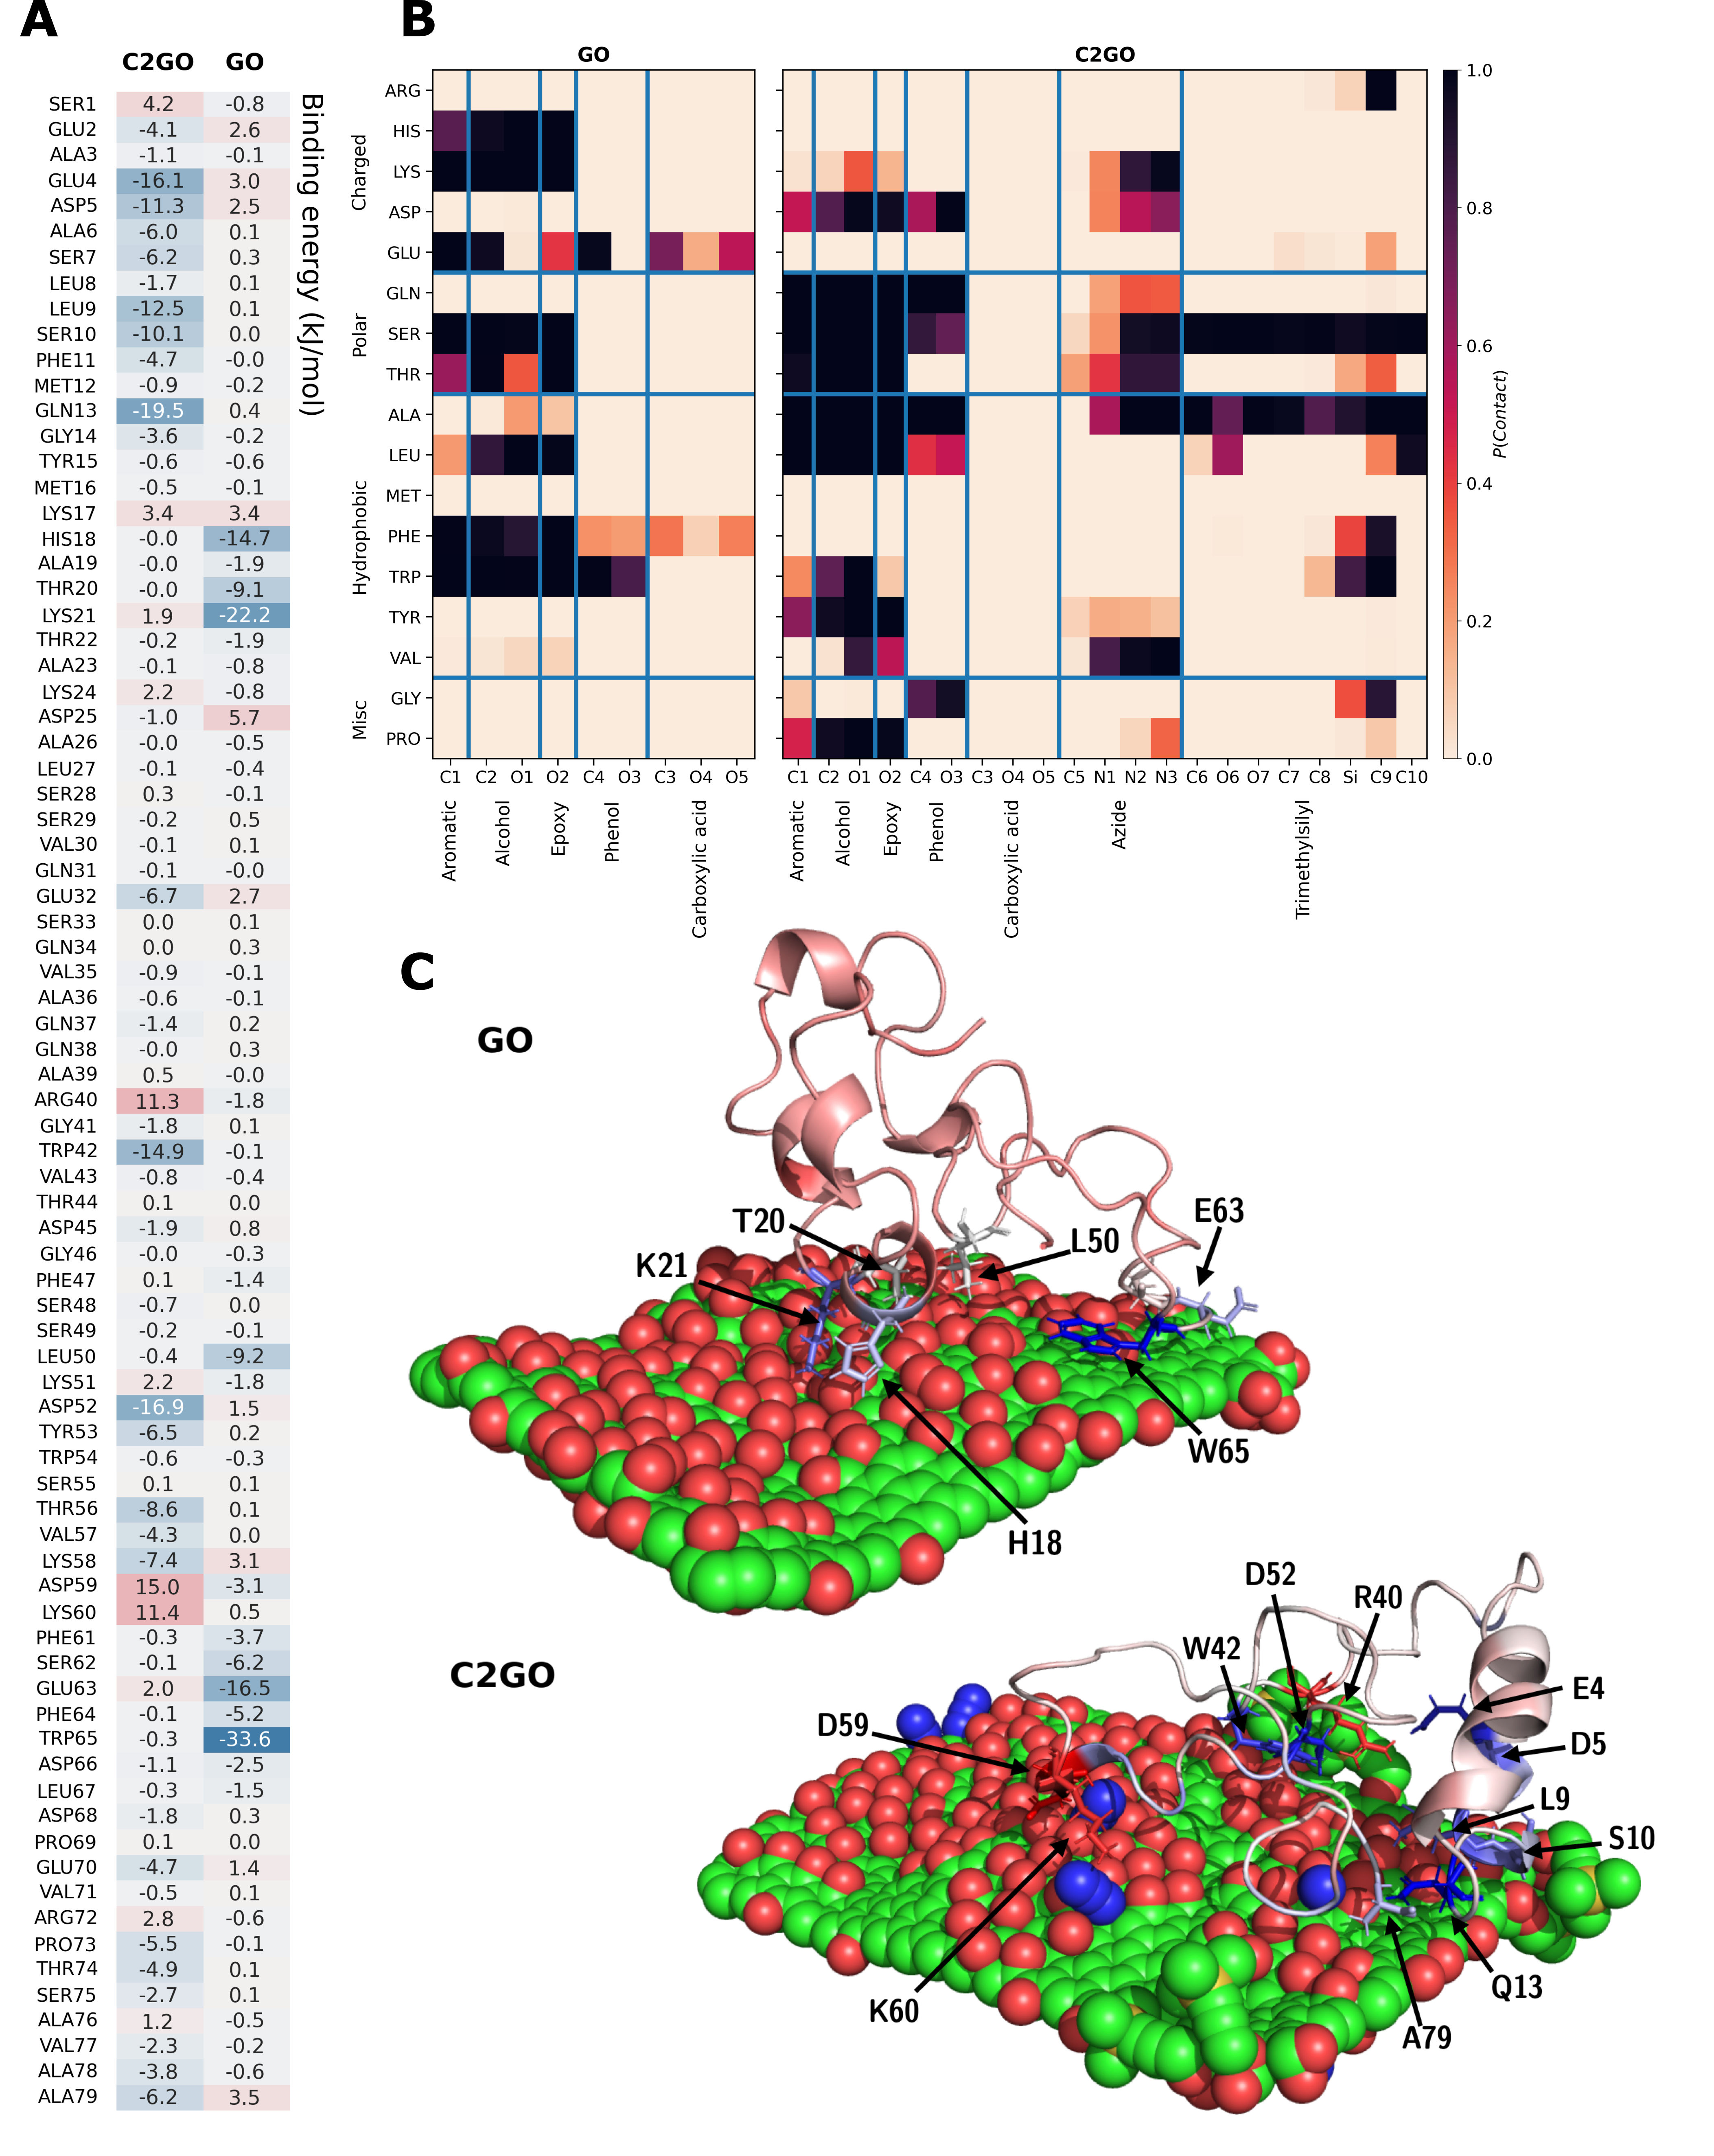
\includegraphics[width=\textwidth]{figures/contacts-energies-fixed.png}
    \caption{MM-PBSA binding energy contributions per apo-c3 amino acid residue for GO and C2GO sheets, colour coded by magnitude (A), heat map showing contact probability of apo-c3 amino acid type with GO and C2GO functional group atoms (B) and adsorbed apo-c3 structure on GO and C2GO, protein amino acids at the graphitic interface are coloured by MM-PBSA binding energy contribution and hydrogen atoms have been omitted for clarity (C).}
    \label{fig:contacts}
\end{figure*}
%
The average binding free energy components for the GO-apo-c3 and C2GO-apo-c3 systems are given in Table 1. The binding free energy components are decomposed to per-residue contributions (Fig.~\ref{fig:contacts}A). In this way we can acquire a better understanding of each amino-acid's contribution to the binding free energy of the protein-nanomaterial complex. Per-residue binding free energy contributions are colour-coded by their interaction strength (blue to red) in the protein structure of the final configuration (Fig.~\ref{fig:contacts}C) for GO and C2GO, where each largely contributing amino acid residue has been illustrated and labelled explicitly. \edit{Note that the entropic contribution to the binding free energy is not calculated using high-throughput methods such as g\_mmpbsa, due to their computational cost. Therefore, the binding free energies in (Table 1) are computed to evaluate the relative binding free energy instead of the absolute free energy.}\\

The binding of apo-c3 to the graphitic substrate is driven by amino acids with the highest binding affinities from the beginning of the adsorption process. Apo-c3 residues 60-70 initiate binding with GO (Fig.~\ref{fig:mid-dist-to-grap}), most likely due to the high binding affinity of TRP65 to $\pi$-$\pi$ stack with pristine graphene domains on the GO surface, as well as GLU63 binding with positively charged (tertiary alkyl, phenol and carboxylic acid) carbon atoms (Fig.\ref{fig:contacts}A). From 100 ns apo-c3 binding to GO is driven by positively charged (HIS18, LYS21) and polar (THR20) residues (Fig.\ref{fig:contacts}A) interacting with oxygen containing surface functional groups. Accordingly, the binding free energy of GO-apo-c3 has a higher net contribution of electrostatic interactions when compared with C2GO-apo-c3, contributing -208 kJ/mol to the total binding free energy (Table 1). \\

In contrast, binding to C2GO is driven by both of the extreme N- and C-terminal ends of apo-c3, which also have the highest binding affinity to the C2GO substrate according to the MM-PBSA binding free energy analysis. The N-terminus serves as the main binding domain with C2GO, driven by negatively charged (GLU4, ASP5) and polar (SER10, GLN13) residues interacting with a TMS group and positively charged (tertiary alkyl, phenol and carboxylic acid) surface and edge carbon atoms (Fig.~\ref{fig:prot-c2go-contacts}). Meanwhile, charged amino acid residues contribute a net positive change in binding free energy of apo-c3 to C2GO  (Fig.~\ref{fig:contacts}A), stabilising C2GO-apo-c3 binding and a conserved apo-c3 tertiary structure. Charged amino acids are the only residues in apo-c3 that sterically hinder neighbouring amino acids from binding to the C2GO interface, and this is wholly achieved through azide functional groups, with the exception of ARG40 which is sterically hindered by a silanol group. However, the role of azide groups is not exclusively restricted to an agent for steric hindrance of amino acid side chains to the graphitic surface, as they drive the binding of hydrophobic amino acids in the extreme C-terminal end of apo-c3 (Fig.~\ref{fig:contacts}A,B). Unlike GO-apo-c3, C2GO-apo-c3 binding is dominated by van der Waals interactions, contributing $-463.2$ kJ/mol to the total binding free energy (Table 1). \\

\begin{table*}
\caption{Binding energy components from MM-PBSA calculations performed on the MD trajectories of adsorbed apo-c3 on GO and C2GO sheets. Stronger binding components have been highlighted in bold.} \label{table:pbsa}
\resizebox{\textwidth}{!}{\begin{tabular}{SSSSSS}                         \toprule
     {} & {\vdw (kJ/mol)} & {\elec (kJ/mol)} & {\polar (kJ/mol)} & {\apolar (kJ/mol)} & {\binding (kJ/mol)}\\ \midrule
    {GO}      &{-338.8±0.8}&{\textbf{-208.3±1.5}}&{\textbf{422.2±5.5}}&{-31.9±0.1}&{-156.8±5.3} \\ \midrule
    {C2GO}    &{\textbf{-463.2±0.9}}&{-135.7±1.0}&{420.5±3.0}&{\textbf{-47.5±0.1}}&{\textbf{-225.9±2.8}} \\ 
    \bottomrule
\end{tabular}}
\end{table*}
In the case of GO-adsorbed apo-c3 binding is dominated by electrostatic interactions (Table 1) with a locus around two binding hotspots --- LYS21, TRP65 (Fig.~\ref{fig:contacts}A) ---  which stabilises unfolding of the protein. This is due to the enthalpic contribution of this binding outweighing the bond enthalpy of the intraprotein interactions maintaining the tertiary structure. Due to the changes to the apo-c3 native state tertiary structures induced by adsorption, apo-c3 has a significantly higher conformational entropy. The energetic stabilisation of a denatured protein is attributed to the conformational entropy of amino acid side chains, which would be a barrier to recovering the native state tertiary structure.\cite{leach1998exploring} In contrast, the enthalpic contribution in C2GO-adsorbed apo-c3 is more dispersed over the surface (Fig.~\ref{fig:contacts}A) and is on average dominated by weaker (van der Waals) interactions (Table 1), thus the intraprotein interactions maintaining the tertiary structure are not compromised by any energetic spikes caused by strong binding in any location on the complex interface.
\subsection{Protein structure}
Changes to protein structure during adsorption --- leading to protein denaturing or deformation --- are evaluated using secondary structure, intramolecular hydrogen bonding and solvent-accessible surface area (SASA) analyses. Protein native contacts indicate changes in secondary structure due to adsorption, their temporal evolution is calculated using the define secondary structure of proteins (DSSP) algorithm\cite{Kabsch-1983} and protein intra-molecular hydrogen bonds. 
%
\subsubsection{DSSP and hydrogen bonds}
%
To understand the dynamic progression of denaturing in GO-adsorbed apo-c3, DSSP and hydrogen bond analyses indicate the sequential loss of secondary structure and number of intra-molecular hydrogen bonds respectively. The number of protein intramolecular hydrogen bonds over time (Fig.~\ref{fig:dssp}B) complement the DSSP results (Fig.~\ref{fig:dssp}A) at a higher resolution and are invariant to the DSSP algorithm criteria for defining strands, helices or coils. It shows that over time, unlike C2GO-adsorbed apo-c3, GO-adsorbed apo-c3 has a dynamic character, sporadically gaining or losing hydrogen bonds. These high spatio-temporal hydrogen bond frequencies stabilise intrachain contacts by recovering the loss of hydrogen bonds, indicating structural reorganisation is taking place during adsorption. \\

Loss of secondary structure in C2GO-adsorbed apo-c3 is transient, with temporary loss of $\alpha$-helix character spanning residues 30-40 (Fig.~\ref{fig:dssp}A). In contrast, GO-adsorbed apo-c3 $\alpha$-helix character is lost irreversibly \edit{for residues 30-35 and 55-60} (Fig.~\ref{fig:dssp}B), concomitantly with the formation of $\beta$-turns whose lifetime range from tens to hundreds of ns and persist throughout adsorption \edit{(Fig.~\ref{fig:dssp}C)}. A decrease of $\alpha$-helices accompanied by an increase of $\beta$-strands elsewhere in the protein is a characteristic observed in experimental secondary-structure analysis of denatured protein libraries using vacuum-ultraviolet circular dichroism.\cite{matsuo2007secondary} Within the initial 150 ns of adsorption, $\alpha$-helices spanning residues 1-10, 30-33 and 40-50 transition to coils (Fig.~\ref{fig:dssp}A). Subsequently at 200 ns, the C-terminus loses it's $\alpha$-helix character in residues 55-65, the lost hydrogen bonds (Fig.~\ref{fig:dssp}B) are recovered through forming $\beta$-turn motifs (Fig.~\ref{fig:dssp}A) and stabilising the apo-c3 protein backbone (Fig.~\ref{fig:dssp}C) for the remainder of adsorption until 400 ns. $\beta$-turns remain stable in a solvated state, potentially serving as recognition motifs of protein-protein interaction,\cite{tyndall2005over} until binding takes place with other proteins. Both L4-S7 and W54-T56 transitioned from an alpha-helix to type-I and type-II $\beta$-turns, respectively, whereas S48-K51 transitioned from a coil to a type II $\beta$-turn. 
\begin{figure*}
    \centering
    \includegraphics[width=\textwidth]{figures/dssp-hbonds-fixed.png}
    \caption{Define Secondary Structure of Proteins (DSSP) algorithm applied to the MD trajectory of apo-c3 adsorption with GO and C2GO (A), the number of intramolecular hydrogen bonds per amino acid residue throughout adsorption (B) and illustration of $\beta$-turns induced in GO-adsorbed apo-c3 following denaturing (residues \edit{L}4-S7, S48-K51 and W54-\edit{V57}), pink and grey structures respectively correspond to the initial and final adsorption conformations (C).}
    \label{fig:dssp}
\end{figure*}
%--------------------------------------
%              CLUSTERING 
%--------------------------------------
\subsection{Clustering}
UMAP dimensionality reduction is a useful approach to map high dimensional data of MD protein backbone coordinates trajectories to a lower dimensional protein configuration space.\cite{mcinnes2018umap-software} This is due to the better performance of UMAP in preserving local and global structure relationships compared with conventional dimensionality reduction techniques such as principle component analysis (PCA) or t-distributed stochastic neighbour embedding (t-SNE). A projection of the high dimensional spatio-temporal MD data into a low-dimensional space is used to identify distinct protein structures, bridging pathways and global relationships between distinct configurations. It is also a practical tool for visualising what is otherwise a vast dataset. \\

The number of clusters in the protein configuration space reflects the number of ensembles the protein backbone adopts, namely the distinct structures of apo-c3 during the entire adsorption process. Using this and the visualisation of protein structures corresponding to each cluster, we can see that apo-c3 has higher structural variance when adsorbing on GO than on C2GO, which have 13 and 10 clusters, respectively (Fig.~\ref{fig:umap}). GO-adsorbed apo-c3 clusters show how the protein sequentially undergoes a process of reorganisation (Fig.~\ref{fig:umap}) driven by interchain hydrogen bonding interactions (Fig.~\ref{fig:dssp}B) due to the binding interactions with the GO surface (Fig.~\ref{fig:contacts}A). \\

The temporal evolution of apo-c3 adsorption follows the cluster numbers in the protein configuration space (Fig.~\ref{fig:umap}). The pathways between clusters are synonymous with the DSSP analysis, corresponding to transitions between configuration states where apo-c3 secondary structure either gains or loses $\alpha$-helix, $\beta$-bridge or coil character. In both cases of GO and C2GO adsorption, the reorganisation process requires transitions to discrete intermediary states (clusters) before converging to a stable complex (Fig.~\ref{fig:umap}). The stable complex may or may not recover its secondary structure following these transitions, corresponding to whether it has or has not been denatured via the adsorption process. This is indeed the case in GO-adsorbed apo-c3, which has undergone drastic structural changes and retains some of its N-terminus (Fig.~\ref{fig:umap}) but loses the C-terminus secondary structure. In contrast C2GO-adsorbed apo-c3 does recover most of its secondary structure, where different cluster pathways transition between the highly conserved native backbone (Fig.~\ref{fig:umap}), which is indicative of binding deformations instead of protein denaturing. Note that the images of the protein backbone annotating the clusters only approximate secondary structure character and are not as accurate as the state-of-the-art characterisation of the secondary structure using DSSP analysis (Fig.~\ref{fig:dssp}). 

\begin{figure*}
    \centering
    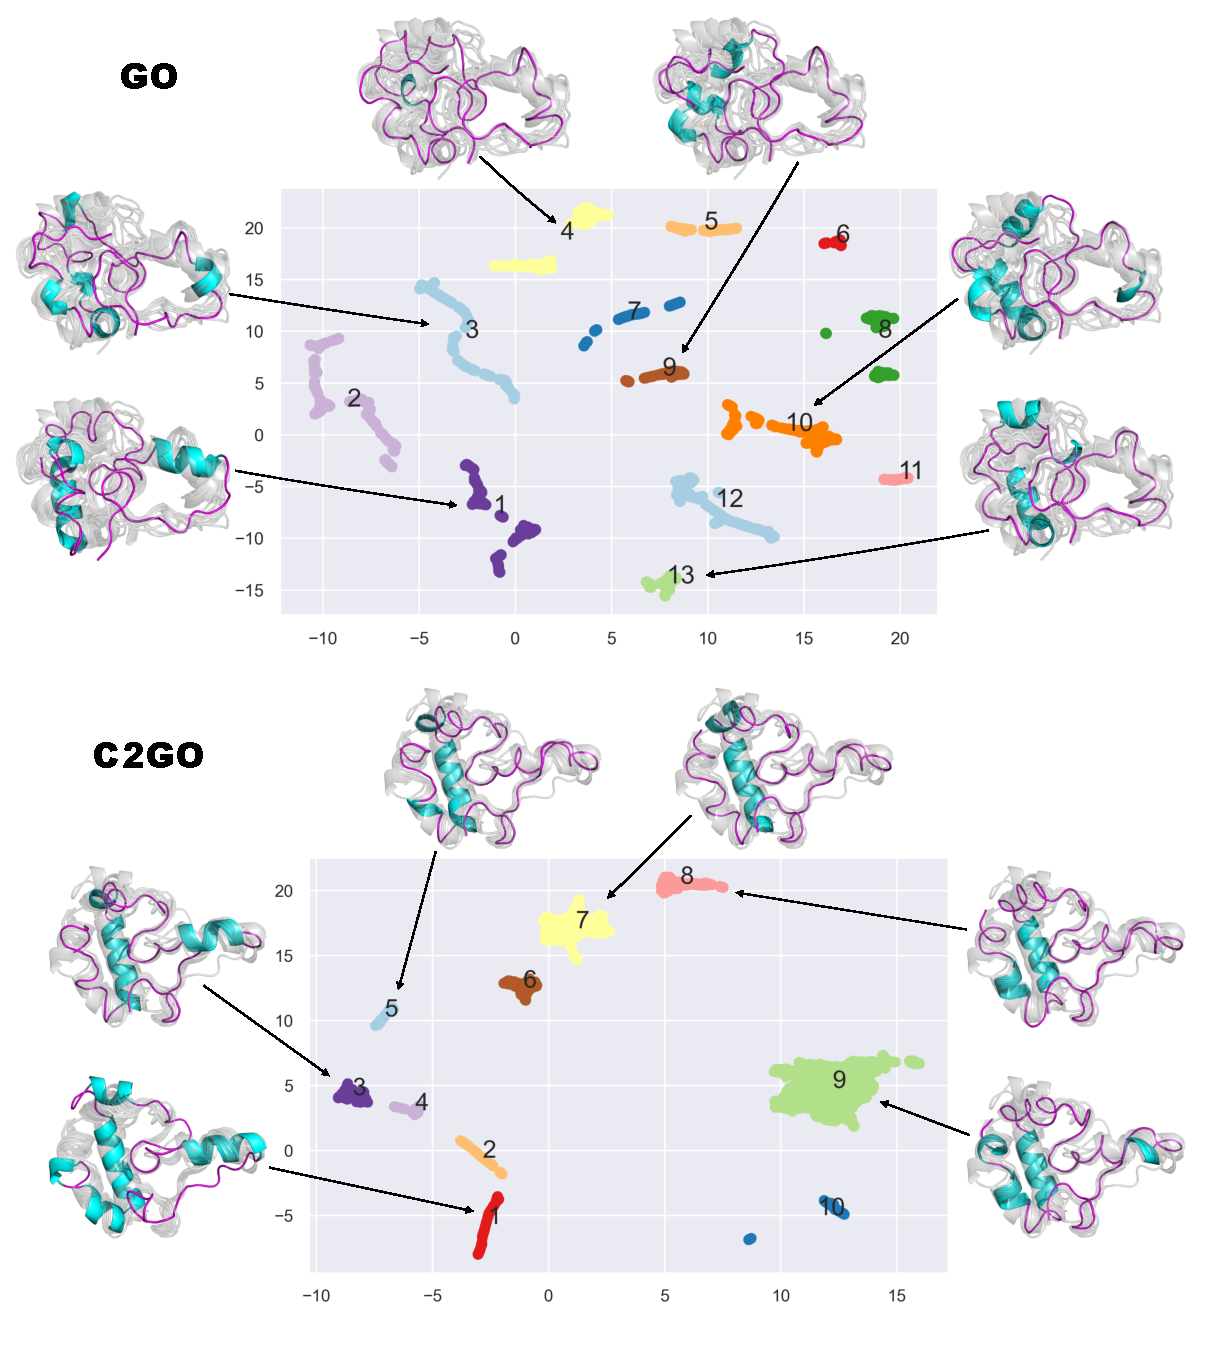
\includegraphics[width=\textwidth]{clustering_both.pdf}
    \caption{Uniform Manifold Approximation and Projection (UMAP) dimensionality reduction of protein backbone denaturing during adsorption on GO (top) and C2GO (bottom) nanosheets. Separate clusters show clear separation of distinct protein backbone secondary structures. Protein structures corresponding to each cluster are coloured by secondary structure (helices in blue, loops in pink) on top of an overlay of all cluster conformations (grey).}
    \label{fig:umap}
\end{figure*}

\subsection{Solvent exposure}
As a result of structural changes induced by adsorption, the hydration of the apo-c3 amino acids change and contribute to potential protein aggregation \textit{in vivo}. As the structure of apo-c3 changes during adsorption on GO, solvent exposure is increased significantly over multiple regions of the amino acid sequence (Fig.~\ref{fig:sasa}A). Some residues will have a larger solvent-accessible surface area (SASA) after adsorption due to change in conformation. Some residues will have a smaller SASA after adsorption either due to a change in conformation leading to new protein-protein contacts or due to interaction of the residue with the nanomaterial in question. There is a correlation with increased solvent exposure in regions where apo-c3 forms $\beta$-turns, as analysed by DSSP and illustrated in (Fig.~\ref{fig:dssp}). The $\beta$-turns remain in this solvated state, potentially serving as recognition motifs for protein-protein interactions until binding to other proteins \textit{in vivo} or \textit{in vitro}.\cite{tyndall2005over} As well as increased solvent exposure of the GO-adsorbed apo-c3 C-terminal helix (residues 47-65), the EVRPTSAVAA minimotif (residues 70-79) has a consistently higher solvent exposure than the native state of apo-c3 in solution (Fig.~\ref{fig:sasa}A,B). These exposed hydrophobic residues keep the adsorbed complex in a disordered state until it can coalesce with its protein/lipid environment. In contrast, the solvent exposure of apo-c3 adsorbed to C2GO is limited to isolated short sequences leaving the conformation of most of the C-terminal helix region (residues 47-65) unchanged (Fig.~\ref{fig:sasa}A).

\begin{figure*}
    \centering
    \includegraphics[width=\textwidth]{sasa-snapshot.png}
    \caption{The surface accessible surface area (SASA) of apo-c3 amino acid residues during adsorption to GO and C2GO sheets, normalised by average SASA of apo-c3 in solution (A) and illustration of exposure of the AVAA minimotif in the C-terminal region of apo-c3 to solvent in GO adsorption and contrasting structure in C2GO adsorption, the nanomaterials are represented as a surface for clarity (B).}
    \label{fig:sasa}
\end{figure*}

Previous work has found that the C-terminal region of apo-c3 is essential for mediating lipid binding, with the N-terminal region (residues 1-40) playing a limited secondary role.\cite{sparrow1977lipid, meyers2017aromatic, lambert1996effect} Solvent exposure analysis of the C-terminal helix expresses the conservation of its lipid-binding function from a physio-chemical perspective. These results may in part delineate the experimentally observed preferential uptake of corona-coated C2GO to corona-coated GO by J774 cells.\cite{mei2018protein} 
%--------------------------------------
%               METHODS 
%--------------------------------------
\section{Methods}
\subsection{Nanomaterial structure}
%
We have modified a Python package \cite{make-graphitics-github} to generate azide and trimethylsilyl (TMS)-alkyne functional group conjugated rectangular graphene-oxide flakes.\cite{albadri2020accurate-github} The package improves on the commonly applied protocol, of randomly placing oxidised functional groups, which we now know is an incomplete model of graphene-oxide structure.\cite{al2020accurate, mouhat2020structure} Instead, we recreate the two-phase nature of oxidised and unoxidised graphene domains observed in microscopy experiments \cite{Pacile2011, Cai2008, Saxena2010, Erickson2010} in accordance with our recent study of accurate large scale modelling of graphene oxide.\cite{al2020accurate}
\subsection{Molecular Dynamics}
%
MD simulations were performed in GROMACS version 2020.1 on the ARCHER2 AMD EPYC Zen2 (Rome) 64 core CPUs at 2.2 GHz or Nvidia V100 GPUs. The all-atom OPLS forcefield was used to simulate the classical simulations. A position restraint algorithm was applied to all non-solvent atoms during equilibration. The $\sim$130\,\AA\, cubic simulation box was fully solvated with TIP3P water molecules. The system net charge was neutralised by adding four sodium ions into the system. The system was relaxed energetically using steepest-descent energy minimisation for 50000 steps with an energetic step size of 0.01 kJ/mol. The minimisation was terminated after the maximum energetic contribution was lower than a threshold of 1000.0 kJ/mol/nm. NVT and NPT equilibration was performed for 100 ps using two separate modified velocity-rescaling thermostat --- with a stochastic term to ensure generating the canonical ensemble --- coupling temperature to velocities for graphene and solvent molecules (NVT),\cite{bussi2007canonical} where a temperature of 300K was maintained and 1 bar using the Parrinello-Rahman barostat (NPT). The Verlet cut-off scheme was employed to generate pair lists and the electrostatic interactions were calculated using the Particle-Mesh Ewald algorithm. Both electrostatic and van der Waals interactions were cut off beyond 1.2 nm. All bonds involving hydrogen atoms were constrained using the LINCS algorithm. Production simulations were run for 400 ns using a timestep of 1~fs. Analysis was performed using the MDAnalysis package \cite{mda, oliver_beckstein-proc-scipy-2016, Michaud-Agrawal-2011} and its analysis modules.\cite{araya2014characterization,smith2019interaction} To identify hydrogen bonds we used the hydrogen bond analysis tool \cite{smith2019interaction} implemented
in MDAnalysis. We used the MDTraj \cite{McGibbon2015MDTraj} implementation of DSSP. 

\subsection{Contact maps}
Contact maps between apo-c3 and the graphitic sheets were calculated using a hard cutoff of \SI{5.0}{\angstrom} between any two heavy (non-hydrogen) atoms. Data over the final \SI{50}{\nano\second} were used for the contact maps, as during this period apo-c3 was stably adsorbed to both GO and C2GO. We constructed contact maps between between GO/C2GO and each specific residue of apo-c3 (Fig.~\ref{fig:prot-go-contacts} and \ref{fig:prot-c2go-contacts}), as well as contact maps between GO/C2GO and each amino acid regardless of its position in the sequence (Fig.~\ref{fig:contacts}B).
%
\subsection{PBSA binding energies}
We post process the last \SI{10}{\nano\second} of MD trajectories using molecular mechanics with Poisson–Boltzmann and surface area solvation (MM-PBSA) analysis implemented using g\_mmpbsa,\cite{kumari2014g_mmpbsa} to obtain a relative order of binding of apo-c3 to the different graphitic nanosheets. The energetic components of the binding free energy are the changes in the system potential energy \textit{in vacuo}, the polar and non-polar solvation energies. The potential energy accounts for bonded (bond, angle and torsion) and non-bonded (van der Waals and electrostatic) energetic terms. Polar solvation energy is the electrostatic contribution to the solvation free energy and is estimated using the Poisson-Boltzmann equation. The non-electrostatic contribution to the solvation free energy accounts for forces between solute and solvent, which are calculated using the solvent accessible surface area (SASA).\cite{kumari2014g_mmpbsa} 
%
\subsection{UMAP dimensionality reduction}
We used the atomic coordinates of apo-c3 to obtain an ensemble of distinct structural conformations when adsorbed to the graphitic sheets. We first centre and align the structures along their backbone atoms, using every tenth frame (\SI{50}{\pico\second}) from the trajectory. We then use the uniform manifold approximation and projection for dimension reduction (UMAP\cite{mcinnes2018umap-software}) algorithm to embed the atomic coordinates of heavy atoms of apo-c3 into a two-dimensional space. UMAP constructs a graph of the points in the high-dimensional space, then optimises a low-dimensional representation of the graph such that the topological distance is preserved to a degree in the embedding.\cite{mcinnes2018umap-software} Therefore, similar conformations that are close in the high-dimensional space will also be close in the reduced space. We set the \code{n\_neighbours} and \code{min\_dist} hyperparameters to 15 and 0.0, respectively, with the latter being a requirement if the points in the reduced space are to be clustered. We use HDBSCAN\cite{mcinnes2017hdbscan}, implemented in scikit-learn\cite{scikit-learn}, to cluster the apo-c3 conformations in the embedded space. We identify representative structures of each conformation by calculating the mean structure of a conformation, then finding the structure with the smallest RSMD from this mean structure.
%
\subsection{SASA solvent exposure}
To quantify the solvent exposure of amino acids during adsorption, we calculated the solvent accessible surface area of each residue of apo-c3 over time. To understand how the conformational changes lead to exposure of residues that are buried in the native state, we normalised the SASA time-series by the mean SASA of each residue of the protein in solution. We used the final \SI{50}{\nano\second} of apo-c3 solution for determining the mean SASA of each residue. Values greater than and less than \num{1} indicate, respectively, increased and decreased exposure to the solvent (Fig.~\ref{fig:sasa}A). The SASA was calculated using the ``rolling-ball" Shake-Rupley algorithm,\cite{SHRAKE1973} implemented in MDTraj.\cite{McGibbon2015MDTraj} This approximates the SASA by effectively rolling a ball over each atom of the protein to define a surface, then examining how much of the each atom's surface is exposed to solvent as opposed to overlapping with surfaces of neighbouring atoms. The radius of the probe in typically set to \SI{1.4}{\angstrom} --- approximately the radius of a water molecule.


%--------------------------------------
%             CONCLUSIONS 
%--------------------------------------
\section{Conclusions}

 This work has dissected the protein structural changes induced by interactions of functional groups and protein residues on the bio-nano interface. Through adsorption on GO, apo-c3 shows denaturing of the secondary structure over large swathes of the protein sequence. Whereas C2GO-adsorbed apo-c3 has limited deformation, with most variance displayed in the N-terminus. The C-terminus of apo-c3 has previously been found to be responsible for lipid binding, with the N-terminus playing a limited secondary role.\cite{sparrow1977lipid, meyers2017aromatic, lambert1996effect} These findings correlate with experimental evidence of the increased cellular uptake of C2GO, as compared to GO, hard protein corona.\cite{mei2018protein} \\

Apo-c3 is found to denature upon adsorption to GO, according to solvent exposure, DSSP and conformational clustering analyses. Following adsorption on GO, apo-c3 forms 3 separate $\beta$-turns that serve as binding motifs for protein-protein interactions. These can aid in subsequent aggregation of serum proteins to the corona, contributing to the corona identity in vivo, hence complicating the targetability of the nanomaterial-corona complex. \\

The functional groups at the binding interface between the nanomaterials and apo-c3 set off a series of dynamic events that result in large-scale secondary structure changes. Contact distances, heatmaps and binding free energy calculations collectively describe the driving forces of the changes in protein structure following adsorption. The introduction of azide and TMS functional groups was sufficient to stop the denaturing of apo-c3 and the formation of $\beta$-turns that serve as protein-protein interaction binding motifs. We find that contact with azide functional groups correlate strongly with contact to other surface functional groups and therefore work cooperatively to maximise the binding surface at the bio-nano interface. Consequently, the C2GO-adsorbed protein is stabilised and is not pushed to structural deformation as is the case in GO-adsorbed protein. The results from this analysis pipeline suggest the causes of protein aggregation and cellular uptake are mediated by the aforementioned changes in protein structure. \\

This work indicates that the dynamic and functional role of adsorbed proteins may be a more important probe to understanding the protein corona, rather than quantifying a static image of its constituent proteins. MD simulations are a valuable tool for such an investigation and our analysis pipeline serves as a transferable method for understanding the structure/function relationship of dynamic protein-nanomaterial adsorption.

%Analysis methods are outlined in the SI, including contact maps (Supp. Note 1), MM-PBSA binding energy calculations\cite{kumari2014g_mmpbsa} (Supp. Note 2), UMAP dimensionality reduction\cite{mcinnes2017hdbscan, scikit-learn} and HDBSCAN clustering\cite{mcinnes2017hdbscan} (Supp. Note 3) and SASA solvent exposure\cite{SHRAKE1973, McGibbon2015MDTraj} (Supp. Note 4).
%\section*{Supplementary figures}
%
\begin{figure}[ht!]
    \centering
    \includegraphics[width=0.8\linewidth]{SI_min-dist-to-grap.png}
    \caption{Minimum distance to any GO/C2GO heavy atom for each residue in apo-C3.}
    \label{fig:mid-dist-to-grap}
\end{figure}

\begin{figure}
    \centering
    \includegraphics[height=18cm]{SI_go-OPLS-R1-residues-condensed_P01.png}
    \caption{Contact probability between each apo-C3 residue and each atom type of GO. Data from the final \SI{50}{\nano\second} of the trajectory. For clarity, only those residues with $P(\mathrm{Contact}) \geq 0.1$ for either GO or C2GO are shown.}
    \label{fig:prot-go-contacts}
\end{figure}

\begin{figure}
    \centering
    \includegraphics[height=18cm]{SI_c2go-OPLS-R2-residues-condensed_P01.png}
    \caption{Contact probability between each apo-C3 residue and each atom type of C2GO. Data from the final \SI{50}{\nano\second} of the trajectory. For clarity, only those residues with $P(\mathrm{Contact}) \geq 0.1$ for either GO or C2GO are shown.}
    \label{fig:prot-c2go-contacts}
\end{figure}

% \chapter{Allosteric regulation of the SARS-CoV-2 main protease}\label{Corona}

%\begin{center}
%    \textit{The contents of this chapter are under review with the Proceedings of the National Academy of Sciences (PNAS)}
%\end{center}

During the coronavirus disease 2019 (COVID-19) pandemic, the scientific community widely attempted to assist in the characterisation of potential therapeutics for the treatment of the disease. With the help of efforts to crystallise SARS-CoV-2 proteins, the molecular dynamics community was able to study structures of SARS-CoV-2 viral proteome. In this work, we were able to identify a method to computationally accelerate the disruption of the catalytic dyad in the SARS-CoV-2 main protease. The mechanism of dyad disruption is an important factor to identifying an inhibitor for the SARS-CoV-2 main protease, the implementation of the metadynamics bias applied in this work can greatly reduce the simulation times of continuing drug discovery efforts. 

\edit{Contributions for this work are as follows: \textbf{Mohamed Ali al-Badri} and \textbf{Khaled Abdel-Maksoud} conceived and planned the research. \textbf{Mohamed Ali al-Badri} performed the molecular dynamics calculations. \textbf{Khaled Abdel-Maksoud} performed the metadynamics calculations. \textbf{Mohamed Ali al-Badri, Khaled Abdel-Maksoud, Christian D. Lorenz} and \textbf{Jonathan W. Essex} analysed the data and \textbf{Mohamed Ali al-Badri} and \textbf{Khaled Abdel-Maksoud} prepared the final manuscript.}
%
%Contributions for this work are as follows: \textbf{Mohamed Ali al-Badri}: \edit{MD simulations}, Conceptualisation, Methodology, Software, Validation, Formal analysis, Investigation, Writing - original draft, Visualization. \textbf{Khaled Abdel-Maksoud}: \edit{Metadynamics simulations}, Conceptualisation, Methodology, Software, Validation, Formal analysis, Writing - original draft, Visualization. 
\clearpage

The Coronavirus Disease of 2019 (COVID-19) is caused by a novel coronavirus known as the Severe Acute Respiratory Syndrome coronavirus 2 (SARS-CoV-2). The main protease (\mpro\!\!) of SARS-CoV-2 mediates viral replication through proteolytic activity and the subsequent generation of infectious virus particles. Current computational efforts towards SARS-CoV-2 \mpro inhibitor design generally neglect an allosteric mechanism linked to His41-Cys145 catalytic dyad disruption and thus do not target the open conformational state. We identify that the orientation of the His41 imidazole side chain away from Cys145 entails an allosteric mechanism for mediating \mpro activity. In this work, we show that molecular dynamics and metadynamics simulations are fundamental for performing computer-aided \mpro inhibitor design where the sampling of this allosteric mechanism within a computationally feasible timescale is essential. We calculate a $4.2 \pm 1.9$ kJ/mol free energy difference between the open and closed states of the SARS-CoV-2 \mpro active site, indicating that favourable ligand interactions with His41 over the Cys145-His41 dyad interaction can stabilise the open state.

\section{Introduction}
Coronaviruses have proven to be a challenge for drug discovery since Severe Acute Respiratory Syndrome Coronavirus 1 (SARS-CoV-1), better known as SARS (2002-2004) and the Middle East Respiratory Syndrome (MERS-CoV) (2012-2013). Severe acute respiratory syndrome coronavirus 2 (SARS-CoV-2) is the cause of the coronavirus disease 2019 (COVID-19). It is a positive-sense single-stranded RNA virus that is contagious in humans, with zoonotic origins and genetic similarities to bat coronaviruses.\cite{andersen2020proximal} The virus mainly enters human cells through the receptor angiotensin converting enzyme 2 (ACE2).\cite{shang2020structural} \\

To date, more than 21 million cases of COVID-19 have been confirmed, with more than 760,000 deaths worldwide.\cite{whoreport} SARS-CoV-2 has a combination of high transmissibility, longer incubation period and a much shorter interval between symptom onset and maximum infectivity when compared with SARS and MERS-CoV.\cite{petersen2020comparing} As a result, even with a relatively low mortality rate, COVID-19 is proving much harder to eradicate and will therefore remain an epidemiological problem until a therapeutic agent is developed.\\

Broad spectrum antiviral medication such as remdesivir have been proposed to decrease SARS-CoV-2 RNA production, however remdesivir was not associated with statistically significant clinical benefits.\cite{wang2020} Recent clinical research has shown that administration of dexamethasone\cite{dexamethasone} or systemic corticosteroids,\cite{steroids} were found to be associated with lower 28-day all-cause mortality when compared with usual care or placebo. \\

The most promising tools for the cessation of the epidemic spread of COVID-19 are vaccines, with many in latter stages of clinical trials, that are expected to be available in late 2020 or early 2021.\cite{world2020draft} The majority of these vaccines are based on platforms such as inactivated viral vectors or RNA sequences encoding the spike glycoprotein of SARS-CoV-2 that trigger an immunogenic response. The SARS spike protein has been identified as the major target of selective pressure in the adaptive evolution of SARS coronaviruses.\cite{zhang2006adaptive} Recently, molecular dynamics (MD) simulations have been used to study the druggability of the SARS-CoV-2 spike.\cite{RommieCasalino} They have identified vulnerabilities in the spike glycan shield --- utilised to frustrate an immune response --- that can be harnessed for vaccine development.\\

Protease inhibitors, however, do not depend on an immunogenic response to elicit immunity. Unlike immunogenic approaches, any inhibitor identified for the SARS-CoV-2 \mpro would very likely also serve as an inhibitor of further evolution of this virus as the sequence and structure of the \mpro are closely related to those from other betacoronaviruses.\cite{ullrich2020sars} Elsewhere, protease inhibitors have been extensively used for the treatment of HIV-AIDS\cite{durrant2011molecular,deeks1999hiv} and hepatitis-C\cite{lamarre2003ns3}. Molecular dynamics (MD) simulations were paramount in identifying the dynamic bound and free states of the HIV-1 protease flaps (two glycine-rich $\beta$-hairpins) that cover a large substrate-binding pocket used as a target for antiviral drugs.\cite{york1993molecular} Also, MD simulations were integral in identifying a cryptic trench within the HIV integrase, which became the target for the first FDA approved HIV integrase inhibitor (raltegravir).\cite{schames2004discovery,durrant2011molecular}\\

The SARS-CoV-2 \mpro is largely responsible for the proteolytic processing of the polyproteins transcribed by the SARS-CoV-2 genome, which are responsible for viral transcription and replication. \mpro cleaves the polyproteins at 11 conserved sites using the catalytic dyad.\cite{hegyi2002conservation, jin2020structure} A catalytic dyad is a set of two coordinated amino acids, common to some enzyme active sites. Within a histidine-cysteine (His-Cys) dyad, the His amino acid will act as a base and activate the Cys mercaptan as a nucleophile for polypeptide cleavage. \\

Owing to the high sequence similarity, the conservation of primary structure about the catalytic sites and the high degree of tertiary structure similarity between both proteases, it has been surmised that the His41-Cys145 catalytic dyad plays the same role of regulating protease activity within both SARS-CoV \mpro proteins.\cite{jin2020structure, ullrich2020sars} Disrupting this dyad, then, disables \mpro activity and subsequent virus replication. In order to be able to cleave the SARS-CoV-2 polyprotein, hydrolysis must be facilitated by priming the \mpro Cys145 mercaptan group for nucleophilic attack via deprotonation by the His41 imidazole group. The proteolytic mechanism in the SARS-CoV \mpro active site regulates protease activity through activation of the Cys145 mercaptan. The rotation of the His41 imidazole towards Cys145 serves as an allosteric trigger to inducing proteolytic activity in SARS-CoV \mpro. One way to disrupt the proteolytic mechanism is to induce a conformational change in the more flexible His41 imidazole side chain of the dyad \edit{a}nd prevent it from abstracting a proton from the Cys145 mercaptan group. An inhibitor would serve to stabilise this disrupted conformation and therefore inhibit \mpro activity.\\

Recently, MD simulations have been used to study the druggability of the SARS-CoV-2 \mpro\!\!.\cite{macchiagodena2020identification, ghahremanpour2020identification} However, conventional MD fails to disrupt the \mpro catalytic dyad and thus deactivate \mpro activity within computationally achievable timescales. As such, screening potential ligands from vast drug libraries to inhibit \mpro is inaccurate and could fail to identify potent inhibitors. Instead, metadynamics (MetaD) enhances the sampling of rare events to reconstruct the free energy landscape by discouraging revisiting of sampled states. It is a useful tool for studying mechanisms of drugs binding to flexible targets where conventional MD may otherwise fail to ergodically sample the free energy landscape. Defining the free energy landscape of a complex simulation is non-trivial and depends on a choice of a few collective variables (CV).\cite{laio2008metadynamics} Other enhanced sampling techniques (Gaussian accelerated MD\cite{gamd}) have been applied in elucidating cryptic pockets not detectable from the \mpro crystal structure, identifying additional pockets for studying \mpro inhibition beside the active site.\cite{sztain2020elucidation}\\

% ----------------------------------------------------------------------
In this work, we apply MetaD to identify the allosteric mechanism of SARS-CoV-2 \mpro using the inhibition of SARS-CoV-1 \mpro with a previously identified potent inhibitor (D3F)\cite{d3f} (Fig.~ \ref{fig:structures}A). In order to comprehensively study whether a contender ligand successfully inhibits the SARS-CoV-2 \mpro\!\!, the \mpro allosteric mechanism must be sampled within feasible timescales. This sampling is difficult to achieve using conventional computational methods as there is a high free energy cost to dyad disruption that these approaches cannot account for. We show that the allosteric mechanism can be sampled using MetaD simulations through biasing rotations about a single dihedral within the dyad, and illustrate this by incorporating a contender ligand (LIG) (Fig.~\ref{fig:structures}B) to SARS-CoV-2 \mpro\!\!.

\begin{figure}
\centering
\includegraphics[width=0.6\linewidth]{lig.png}
\caption{Inhibitor candidate ligand structures with molecular weight (MW) and calculated lipophilicity (LogP). (A) D3F, a strong binder and inhibitor of SARS-CoV-1 \mpro\!\!. (B) The drug candidate (code named LIG herein) considered for binding and inhibition of SARS-CoV-2. LogP values were calculated using the ChemDraw LogP estimation tool.}
\label{fig:structures}
\end{figure}


\section{Results}
%
\subsection{Allosteric regulation of SARS-CoV-1 and SARS-CoV-2 \mpro activity is linked to the His41-Cys145 interaction}

Co-solvent MD simulations \cite{seco2009binding} are a useful tool for identifying binding hotspots on protein surfaces by simulating proteins in a solution of water and co-solvent molecules. This dynamic approach to identifying binding sites incorporates proteins' inherent flexibility, allowing the cosolvent molecules to compete with water to bind to the protein surface.\cite{ghanakota2016driving} Our co-solvent MD simulations were initiated by placing five LIG molecules randomly surrounding SARS-CoV-2 \mpro. Of the five LIG molecules, only one entered the binding site of SARS-CoV-2 in order to stabilise a binding mode (Fig.~\ref{fig:bound_structures}). \\

A short simulation of SARS-CoV-1 \mpro with the inhibitor D3F bound in the active site was also performed and was used to evaluate the success of the observed LIG binding in inhibiting SARS-CoV-2 \mpro\!\!, as the initial D3F binding mode has been proven to successfully inhibit SARS-CoV-1 \mpro in previous studies.\cite{d3f} When observing the bound state of D3F to SARS-CoV-1 \mpro\!\!, the nitrate group most proximal to His41 forms a strong electrostatic interaction between a D3F nitro O atom and the N1-H of the His41 imidazole (D3F N-O $\cdot\cdot\cdot$ H-N1 His41) (Fig.~\ref{fig:bound_structures}A). This interaction stabilises the orientation of His41 away from Cys145 which comprises the open (``holo") conformation of \mpro\!\!. Despite the ligand appearing as bound within the SARS-CoV-2 \mpro active site, His41 is not seen to interact with the bound ligand at all (Fig.~\ref{fig:bound_structures}B). The primary difference between the binding modes of D3F to SARS-CoV-1 \mpro and LIG to SARS-CoV-2 \mpro is the orientation of the His41 imidazole with respect to Cys145. In the latter case, the His41-Cys145 catalytic dyad is maintained and thus the \mpro is within a closed (``apo") conformation. The disruption of the catalytic dyad via reorientation of the His41 imidazole or interaction with the Cys145 mercaptan side chain\cite{jin2020structure} therefore serves as a prospective diagnostic tool for successful inhibition.
%
\begin{figure}
    \centering
    \includegraphics[width=\linewidth]{figures/side_by_side_labeled.pdf}
    \caption{The observed binding modes of (A) D3F (yellow) within the SARS-CoV-1 \mpro catalytic binding site (cyan), showing the disrupted catalytic dyad (``holo") and the strong D3F interaction with His41 (dashed red line) and (B) LIG (orange) within the SARS-CoV-2 \mpro catalytic binding site (pink) with a maintained catalytic dyad (``apo"). The dyad residues and their interactions (dashed blue line) are labeled His41 and Cys145.}
    \label{fig:bound_structures}
\end{figure}
\subsection{Generating the SARS-CoV-2 \mpro active state via His41 side chain reorientation}
%
The disruption of the catalytic dyad to promote ligand binding was further explored through the use of enhanced sampling simulations. The binding mode of D3F to SARS-CoV-1 \mpro indicates an ability to achieve inhibition of SARS-CoV-2 \mpro through promoting interactions with the His41 imidazole in the holo form. Metadynamics (MetaD) is herein employed with a bias potential over the \dihone dihedral of His41 in order to induce rotation of the His41 side chain imidazole group about the \dihtwo dihedral. The \dihtwo dihedral cannot be used as a CV due to an intrinsic conformational restriction, since the dihedral is part of the protein backbone. Instead, we have applied a bias to the \dihone dihedral torsion, which allows us to investigate the free rotational orientation of the His41 side chain imidazole (Fig.~\ref{fig:dihedrals}).\\
%
\begin{figure}
  \centering
  \begin{tabular}{@{}p{0.5\linewidth}@{\quad}p{0.5\linewidth}@{}}
    \subfigimg[width=\linewidth]{\large{\textbf{A} \quad $\mathbf{\xi_{1}}$ dihedral }}{chi1} &
    \subfigimg[width=\linewidth]{\large{\textbf{B} \quad $\mathbf{\xi_{2}^{backbone}}$ dihedral}}{chi2}
  \end{tabular}
  \caption{His41 imidazole side chain dihedrals. (A) \dihone dihedral used for construction of the MetaD bias. (B) \dihtwo dihedral considered within analysis of the performance of the bias and characterising the disassociation of His41 from Cys145.}
\label{fig:dihedrals}
\end{figure}

Ergodic sampling along the \dihone torsional CV space was achieved using MetaD simulations. The free energy surface with respect to the \dihone dihedral was calculated and is shown in (Fig.~\ref{fig:freeenergy_convergence}, top). This surface was used to verify metadynamics convergence by evaluating the relative free energy differences between pairs of free energy minima, which stabilised after 70 ns (Fig.~\ref{fig:freeenergy_convergence}, bottom).


\begin{figure}
    \centering
    \includegraphics[width=\linewidth]{MetaDFES_segments.png}
    \includegraphics[width=\linewidth]{MetaDFES_convergence.png}
    \caption{\edit{Analysis of convergence of His41 imidazole dihedral MetaD bias potential. Potential of mean force (PMF) projected on the \dihone dihedral space of the bias potential. Relative free energy differences (in kJ/mol) were calculated between minima indicated by the dashed lines (top). Relative free energy difference between each pair of minima defined within the above PMF over the simulation time (bottom).}}
    \label{fig:freeenergy_convergence}
\end{figure}


\subsection{\mpro catalytic dyad conformational changes}

In order to verify that our choice of CV of \dihone torsion couples to and changes the degree of \dihtwo torsion, we compare the probability densities found from our MetaD simulation to the probability distributions observed in our co-solvent MD simulations of LIG-SARS-CoV-2 and the D3F-SARS-CoV-1, which we use as the ``apo" (closed conformation) and ``holo" (open conformation) states, respectively. In (Fig.~\ref{fig:1Dim_PDF}A), the MetaD probability distribution clearly samples both ``apo" and ``holo" states. In (Fig.~\ref{fig:1Dim_PDF}B), this choice of \dihone torsion CV also biases the the catalytic dyad into an open state by orienting the His41 imidazole away from Cys145, measured through the (His41-N$_{\epsilon2}$)-(Cys145-S$_{\gamma}$) distance.\\

\begin{figure}
    \centering
    \includegraphics[width=0.8\linewidth]{MetaDPMF.png}
    \caption{1D probability density functions obtained from the co-solvent MD simulations of SARS-CoV-1 ``holo" (blue), SARS-CoV-2 ``apo" (green) and SARS-CoV-2 MetaD simulation (purple) over the (A) \dihtwo dihedral space and (B) (Cys145-S$_{\gamma}$)-(His41-N{$\epsilon$}) distance.} 
    \label{fig:1Dim_PDF}
\end{figure}

To demonstrate the interconnection of the \dihtwo torsion and (Cys145-S$_{\gamma}$)-(His41-N{$\epsilon$}) distance, we can represent the sampling of co-solvent MD simulations (``holo" - (Fig.~\ref{fig:2DPMF}A) and ``apo" - (Fig.~\ref{fig:2DPMF}C)) with the interchangeable MetaD sampling of both ``apo" and ``holo" states in a 2D space (Fig.~\ref{fig:2DPMF}B).  Comparing against the three density functions, it is noted that the region about \dihtwo = -0.5 rad overlaps with the ``holo" state, while the region about \dihtwo = 0.5 rad overlaps with the sampled density of the ``apo" in which the catalytic dyad remains intact throughout. This comparison allows for the characterisation of each of the respective regions in the metadynamics density function above to be considered as ``apo" and ``holo" conformational states (Fig.~\ref{fig:2DPMF}B).\\

In (Fig.~\ref{fig:2DPMF}B), the bimodal probability density in the 2D CV space includes points at shorter (Cys145-$S_{\gamma}$)--(His41-N{$\epsilon$}) distances at \dihtwo = -0.5 rad. This region indicates that, in the absence of a potent inhibitor, the ``holo" state cannot be stabilised by biased \dihone sampling alone. As such, the dyad will reorient to maintain the Cys145-His41 side chain interaction.\\

\begin{figure}[h!]
  \centering
  \begin{subfigure}
    \includegraphics[width=0.3\linewidth]{HOLO_2DPMF.png}
  \end{subfigure}
  \begin{subfigure}
    \includegraphics[width=0.3\linewidth]{MetaD_2DPMF.png}
  \end{subfigure}
    \begin{subfigure}
    \includegraphics[width=0.3\linewidth]{APO_2DPMF.png}
  \end{subfigure}
  \caption{Probability density functions of the (A) SARS-CoV-1 ``holo" , (B) SARS-CoV-2 MetaD (inset showing MetaD ``holo") and (C) SARS-CoV-2 ``apo" MD simulation defined within a 2D CV space of the His41 \dihtwo dihedral and the (Cys145-$S_{\gamma}$)-(His41-N{$\epsilon$}) atomic distance.}
  \label{fig:2DPMF}
\end{figure}


To confirm that the choice of a \dihone bias samples the ``apo"--``holo" transition, the time-dependent behaviour of both the \dihtwo dihedral and the (Cys145-$S_{\gamma}$)-(His41-N{$\epsilon$}) distance was evaluated using K-means clustering.\cite{scikit-learn} Three distinct clusters were found (Fig.~\ref{fig:2DAveragePMF}) corresponding to the ``apo" conformation (\dihtwo = 0.5 rad) , ``holo" conformation (\dihtwo = -0.5 rad) and transition region. The time dependent behaviour of \dihtwo dihedral and (Cys145-$S_{\gamma}$)-(His41-N{$\epsilon$}) distance show the choice of CV freely samples the reversible ``apo"--``holo" transition throughout the 100 ns trajectory.\\

\begin{figure}[!h]
    \centering
    \includegraphics[width=\linewidth]{KMeansVsTime_0.png}
    \includegraphics[width=\linewidth]{KMeansVsTime_1.png}
    \caption{\edit{Time evolution of the MetaD simulation trajectory and the associated cluster identity of points with respect to the His41 \dihtwo dihedral (top) and the (Cys145-S$_{\gamma}$)-(His41-N{$\epsilon$}) distance (bottom).}}
    \label{fig:2DAveragePMF}
\end{figure}

\subsection{\mpro free energy surfaces}

In order to verify the reproducibility of the constructed bias, four replicas of the MetaD simulation were performed until convergence was observed in each. The free energy profiles obtained in each of the replicas show agreement, with deviation from the average free energy values observed chiefly at the transition states and at the minimum at \dihone = 1.9 rad. The deviation at this minimum is due to the corresponding state being sparsely sampled in all replicas compared to the other system states as a result of the high free energy barrier restricting sampling from other observed minima (Fig.~\ref{fig:AverageFES}).\\

\begin{figure}[!h]
    \centering
    \includegraphics[width=\linewidth]{AverageFES_4Reps.png}
    \caption{\edit{Mean free energy surface obtained over 4 replicas of His41 torsional metadynamics defined within the \dihone dihedral space. The shaded region corresponds to the standard deviation about each free energy point calculated over the set of replicas.}}
    \label{fig:AverageFES}
\end{figure}

As convergence of the bias was observed for all four replicas, it can be assumed that any sampling beyond the point of convergence is within the desired thermodynamic ensemble. Thus, the mean free energy surface with respect to the His41 \dihtwo dihedral over the 4 replicas was computed (Fig \ref{fig:1DPMFAll_Dihtwo}). The mean surface is bimodal, with positions of the minima at 0.5 and -0.5 rad corresponding the the sampled ``apo" and ``holo" states of the SARS-CoV-2 \mpro catalytic dyad, respectively. The ``apo"-``holo" relative free energy difference of $4.2 \pm 1.9$ kJ/mol ($1.0 \pm 0.5$ kcal/mol) indicates that the ``holo" state is less energetically stable than the ``apo" state in the absence of any ligands interacting with His41. Considering this free energy difference between states and the high free energy barrier ($15.0 \pm 1.3$ kJ/mol / $3.6 \pm 0.3$ kcal/mol) between them, it can be assumed that the dyad ``apo"--``holo" transition is unlikely to be sampled using unbiased conventional MD simulations alone.\\

The free energy surface of SARS-CoV-1 ``holo" (dashed blue line) was computed from the reference simulation of the D3F-SARS-CoV-1 \mpro complex using population analysis (Fig.~\ref{fig:1DPMFAll_Dihtwo}). This surface is used as a reference state to compare against the mean MetaD free energy surface as the ``holo" state. The SARS-CoV-1 ``holo" conformation is more energetically stable than the SARS-CoV-2 MetaD surface ``holo" minimum by approximately $4.2 \pm 1.9$ kJ/mol ($1.0 \pm 0.5$ kcal/mol). This energy difference highlights how the energetic penalty associated with dyad disruption in the ``apo"--``holo" transition may be recovered by ligand interactions in the active site. \edit{All MetaD replicas yielded sampling of the two rotamers of His41 about the backbone dihedral. The larger error about the ``dyad disrupted" conformation at -0.5 rad (Fig.~\ref{fig:1DPMFAll_Dihtwo}) is due to sampling with a ligand-free active site for \mpro\!, meaning that less stable conformation isn't stabilised by ligand interactions unlike the case of D3F binding.}\\

\begin{figure}[!h]
    \centering
    \includegraphics[width=\linewidth]{1DDih2FES_4Reps.png}
    \caption{Mean free energy surface obtained from the MD simulation of D3F-SARS-CoV-1 ``holo" (blue) and four replicas of His41 torsional MetaD simulations (purple), defined within the \dihtwo dihedral space. The shaded region corresponds to the standard deviation about each free energy point calculated over the set of MetaD replicas.}
    \label{fig:1DPMFAll_Dihtwo}
\end{figure}
%
%--------------------------------------
%
%
%
%               METHODS
%
%
%
%--------------------------------------
\section{Methods}

\subsection{Molecular Dynamics}
All MD simulations were performed in GROMACS version 2019.4 on the ARCHER Cray XC30 supercomputer on a single 2.7 GHz, 12-core E5-2697 v2 (Ivy Bridge) series processor node, NVIDIA GeForce RTX 2060 or GeForce GTX1080Ti GPUs with the CUDA 10.2 toolkit.  The AMBER14SB forcefield \cite{amberff14SB} was used to model the system, where ligand molecule forcefield parameters were generated using the General Amber ForceField v2 (GAFF2) with charges calculated using the AM1-BCC semi-empirical method.\cite{amber16}.\\

The structure of the candidate ligand LIG was derived from a virtual fragment expansion, docking, and screening exercise provided by Gabriel Grand, Elana Simon, Michael Bower, Bruce Clapham and Jonah Kallenbach of Reverie Labs.\cite{gabereverie} Protein X-Ray diffraction (XRD) structures for SARS-CoV-1 \mpro holo structure (PDB code: 2GZ7) \cite{2gz7} and SARS-CoV-2 \mpro apo structure (PDB code: 5RE4) were used for these simulations. Missing residues from the SARS-CoV-2 XRD structure were modelled using MODELLER \cite{modeller} and subsequently solvated in a 90 $\rm{\AA}$ cubic box of TIP3P water molecules. \\

For co-solvent MD simulations, five of the candidate ligand (LIG) were placed in random coordinates within the box and the system net charge was neutralised by adding 4 sodium ions into the system. The co-solvent MD simulations was performed for 100 ns. The simulation of D3F bound in SARS-CoV-1 \mpro was performed for 10 ns. The net charge in the system was neutralised by adding 3 sodium ions. In all structures prepared for simulation, the His41 side chain was maintained at the N1-H tautomeric state, as this state is primed for nucleophillic attack from the Cys145 mercaptan in the active catalytic dyad.\\

The system was relaxed energetically using steepest-descent energy minimisation for 50000 steps with an energetic step size of 0.01 kJ/mol. The minimisation was terminated after the maximum energetic contribution was lower than a threshold of 10.0 kJ/mol. NVT and NPT equilibration was performed for 1 ns using two separate velocity-rescaling thermostat coupling temperature to velocities for protein, drug and solvent molecules (NVT), where a temperature of 300 K was maintained and 1 bar using the Parrinello-Rahman barostat (NPT).\cite{parrinello1981polymorphic} The Verlet cut-off scheme was employed to generate pair lists and the electrostatic interactions were calculated using the Particle-Mesh Ewald algorithm.\cite{pme} Both electrostatic and van der Waals interactions were cut off beyond 1.2 nm. All bonds involving hydrogen atoms were constrained using the LINCS algorithm.\cite{hess1997lincs} Production simulations ran with an integration stepsize of 2 fs. MDAnalysis was used to postprocess the MD trajectories for analysis.\cite{mdanalysis1, mdanalysis2}\\

\subsection{Metadynamics}
Four independent replicas of the non-tempered MetaD simulation were run to convergence.\cite{metaD} The bias potential was setup to sample energetically hindered rotations about the \dihtwo dihedral of His41 by biasing the sampling along the \dihone torsional profile directly. The bias was accumulated with a Gaussian deposition rate $\tau = 1$ ps. The deposited Gaussians had a fixed height of 0.1 kJ/mol and employed an adaptive width scheme in which the correlation between the biased CV space and the microscopic configuration space is utilised to recalculate the covariance matrix. A correlation length of 0.5 $\mathrm{\AA}$ was used.\cite{adaptive} MetaD simulations were performed using Plumed 2.5.4.\cite{plumed}. All the data and Plumed input files required to reproduce the results reported in this paper are available on PLUMED-NEST (www.plumed-nest.org), the public repository of the PLUMED consortium \cite{plumed}, as plumID:20.027. 
%--------------------------------------
%
%
%
%               CONCLUSIONS
%
%
%
%--------------------------------------
\section{Conclusions}
We have presented the application of metadynamics to molecular dynamics simulations of the SARS-CoV-2 \mpro to better inform the drug discovery efforts including virtual screening, molecular docking and unbiased molecular dynamics simulations. We show that the proteolytic mechanism of \mpro is contingent on the integrity of the His41-Cys145 catalytic dyad and that the rotation of the His41 imidazole side chain to Cys145 acts as an allosteric trigger to regulating this proteolytic activity.\\

Using metadynamics, we find that promoting ligand binding and sampling of the active site of the protease is achieved through disrupting the catalytic dyad by biasing over the His41 \dihone dihedral to subsequently sample over the \dihtwo dihedral. Using the (Cys145-$S_{\gamma}$)-(His41-N{$\epsilon$}) distance and the \dihtwo dihedral to define the collective variable (CV) space, we identify clusters of unbound, intermediary and bound conformations of the flexible \mpro active site throughout the simulation. We show that repeated replicas of the His41 torsional metadynamics reproduce the free energy surface along the 1D \dihone and \dihtwo spaces. Our results detail the allosteric regulation of the SARS-CoV-2 \mpro\!\!, irrespective of the choice of ligand. The candidate ligand LIG acts as a toy model and its inadequacy in disrupting the catalytic dyad was established by drawing comparisons of its interaction in the \mpro active site against the ligand D3F with SARS-CoV-1 \mpro\!\!.\\

The application of our analysis uncovers the changes on the receptor structure as a result of an allosteric mechanism resolved using enhanced sampling. This observation can assist in selecting an optimal strategy for screening ligands from drug libraries. The free energy comparison between the D3F unbound and bound ``holo" state minima suggests that the energy expended in disrupting the dyad can be readily recovered using ligand interactions in the active site, and so this open dyad state should be considered alongside the closed state as a target for virtual screening. We provide coordinates for structures corresponding to the open catalytic dyad state of SARS-CoV-2 \mpro as supplementary data for use in further studies. 
%\chapter{Allosteric regulation of SARS-CoV-2 protease}
%\label{Corona}
%
%During the coronavirus disease 2019 (COVID-19) pandemic, the scientific community widely attempted to assist in the characterisation of potential therapeutics for the treatment of the disease. With the help of efforts to crystallise SARS-CoV-2 proteins, the molecular dynamics community was able to study protein structures of SARS-CoV-2 components. In this work, we were able to identify a method to computationally accelerate the disruption of the catalytic dyad in the SARS-CoV-2 main protease. The mechanism of dyad disruption is an important factor to identifying an inhibitor for the SARS-CoV-2 main protease, the implementation of the metadynamics bias applied in this work can greatly reduce the simulation times of continuing drug discovery efforts. 
%
%Contributions for this work are as follows: \textbf{Mohamed Ali al-Badri}: Conceptualisation, Methodology, Software, Validation, Formal analysis, Investigation, Writing - original draft, Visualization. \textbf{Khaled Abdel-Maksoud}: Conceptualisation, Methodology, Software, Validation, Formal analysis, Writing - original draft, Visualization. \textbf{Christian D. Lorenz}: Writing - review \& editing, Supervision, Resources. \textbf{Jonathan W. Essex}: Writing - review \& editing, Supervision, Resources.
%
%%\includepdf[pages=-, offset=75 -75]{PDF_PAPERS/KAM_MAB_SARS2.pdf}
%%\includepdf[pages=-, offset=75 -75]{PDF_PAPERS/PNAS_corona_SI.pdf}
%
%\includepdf[pages=-, offset=75 -75,
%    addtotoc={
%     2,section,1,Introduction,covid2,
%     6,section,1,Results,covid6,
%     6,subsection,2,Allosteric regulation of SARS-CoV-1 and SARS-CoV-2 M$^{\rm{Pro}}$ activity is linked to the His41-Cys145 interaction,covid7,
%     7,subsection,2,Generating the SARS-CoV-2 M$^{\rm{Pro}}$ active state via His41 side chain reorientation,covid7,
%    10,subsection,2,M$^{\rm{Pro}}$ catalytic dyad conformational changes,covid10,
%    12,subsection,2,M$^{\rm{Pro}}$ free energy surfaces,covid12,
%    15,section,1,Conclusions,covid15,
%    16,section,1,Methods,covid16,
%    16,subsection,2,Molecular Dynamics,covid16,
%    18,subsection,2,Metadynamics,covid18},
%     addtolist={
%     6, figure,{Inhibitor candidate ligand structures with molecular weight (MW) and calculated lipophilicity (LogP). (A) D3F, a strong binder and inhibitor of SARS-CoV-1 M$^{\rm{Pro}}$. (B) The drug candidate (code named LIG herein) considered for binding and inhibition of SARS-CoV-2. LogP values were calculated using the ChemDraw LogP estimation tool.},b,
%     8, figure,{The observed binding modes of (A) D3F (yellow) within the SARS-CoV-1 M$^{\rm{Pro}}$ catalytic binding site (cyan), showing the disrupted catalytic dyad (``holo”) and the strong D3F interaction with His41 (dashed red line) and (B) LIG (orange) within the SARS-CoV-2 MPro catalytic binding site (pink) with a maintained catalytic dyad (``apo”). The dyad residues and their interactions (dashed blue line) are labeled His41 and Cys145.},c,
%     9, figure,{His41 imidazole side chain dihedrals. (A) $\xi_1$ dihedral used for construction of the MetaD bias. (B) $\xi^{\rm{backbone}}_{2}$ dihedral considered within analysis of the performance of the bias and characterising the disassociation of His41 from Cys145.},d,
%     11,figure,{1D probability density functions obtained from the co-solvent MD simulations of SARSCoV-1 ``holo” (blue), SARS-CoV-2 ``apo” (green) and SARS-CoV-2 MetaD simulation (purple) over the (A) $\xi^{\rm{backbone}}_{2}$ dihedral space and (B) (Cys145-S$_{\gamma}$)-(His41-N$_{\epsilon}$) distance.},e,
%     12, figure, {Probability density functions of the (A) SARS-CoV-1 ``holo”, (B) SARS-CoV-2 MetaD (inset showing MetaD ``holo”) and (C) SARS-CoV-2 ``apo” MD simulation defined within a 2D CV space of the His41 $\xi^{\rm{backbone}}_{2}$ dihedral and the (Cys145-S$_{\gamma}$)-(His41-N$_{\epsilon}$) atomic distance.},f,
%     14, figure, {Mean free energy surface obtained for co-solvent MD simulations of D3F-SARS-CoV-1 ``holo” (blue) and four replicas of His41 torsional MetaD simulations (purple), defined within the $\xi^{\rm{backbone}}_{2}$ dihedral space. The shaded region corresponds to the standard deviation about each free energy point calculated over the set of MetaD replicas.},g}]{PDF_PAPERS/KAM_MAB_SARS2.pdf}
%\includepdf[pages=-, offset=75 -75,addtotoc={
%     1,section,1,Supplementary Figures,pppp1,
%     5,section,1,Supplementary Notes, pppp5,
%     5,subsection,2,Clustering reproducibility, pppp5},
%     addtolist={
%     1, figure,{Analysis of convergence of His41 imidazole dihedral MetaD bias potential. Potential of mean force (PMF) projected on the $\xi_1$ dihedral space of the bias potential. Relative free energy differences (in kJ/mol) were calculated between minima indicated by the dashed lines (top). Relative free energy difference between each pair of minima defined within the above PMF over the simulation time (bottom).},aaaa,
%     2, figure,{Time evolution of the MetaD simulation trajectory and the associated cluster identity of points with respect to the His41 $\xi^{\rm{backbone}}_{2}$ dihedral (top) and the (Cys145-S$_{\gamma}$)-(His41-N$_{\epsilon}$) distance (bottom).},bbbb,
%     3, figure,{Mean free energy surface obtained over 4 replicas of His41 torsional metadynamics defined within the $\xi_1$ dihedral space. The shaded region corresponds to the standard deviation about each free energy point calculated over the set of replicas.},cccc,
%     4,figure,{Probability density profiles of clusters from the aggregate trajectory of four MetaD replicas projected into the 2D CV space comprised of the $\xi^{\rm{backbone}}_{2}$ dihedral and the (Cys145-S$_{\gamma}$)-(His41-N$_{\epsilon}$) distance. Population densities with respect to each CV axis are aligned for each cluster.},dddd}]{PDF_PAPERS/PNAS_corona_SI.pdf}
% \vspace{-1cm}
\chapter{Superexchange mechanism and quantum manybody excitations in the archetypal di-Cu oxo-bridge}
\label{Hemocyanin}
\vspace{-1cm}

In this work, we study the electronic structure of the hemocyanin protein, where in particular we study the 59-atom protein core using density functional theory + dynamical mean field theory (DFT+DMFT). Here, we find that the hemocyanin protein utilises electronic correlation effects in performing its function of oxygen transport. By treating the copper 3\textit{d} electrons in the hemocyanin functional site using DMFT, we recover experimentally observed singlet electronic ground state. This work allows the transferability of the DFT+DMFT approach to the quantum treatment of the entire protein, using linear-scaling DFT. The importance of accurate simulation of the Hemocyanin core is in understanding how biological systems have evolved to function through quantum biology, as well as its use in biomimetic applications in engineering.\cite{al2020superexchange} \edit{Contributions for this work are as follows: \textbf{Cedric Weber} and \textbf{Mohamed Ali al-Badri} conceived and planned the research. \textbf{Mohamed Ali al-Badri, Edward Linscott} and \textbf{Cedric Weber} performed the calculations. \textbf{Mohamed Ali al-Badri
Edward Linscott, Antoine Georges, Daniel J. Cole} and \textbf{Cedric Weber} analysed the data and contributed to the final manuscript. \textbf{Edward Linscott} independently ran the NBO analysis (Supp. Fig.~3) and the scaling calculations (Supp. Fig.~5).}

%Contributions for this work are as follows: \textbf{Cedric Weber and Mohamed Ali al-Badri} conceived and planned the research. \textbf{Mohamed Ali al-Badri, Edward Linscott} and \textbf{Cedric Weber} performed the calculations. \textbf{Mohamed Ali al-Badri, Edward Linscott, Antoine Georges, Daniel J. Cole} and \textbf{Cedric Weber} analysed the data and contributed to the final manuscript. \edit{Edward Linscott independently ran the Natural Bonding Orbital (NBO) analysis (Supplementary Fig.~3) and the scaling calculations (Supplementary Fig.~5).}
%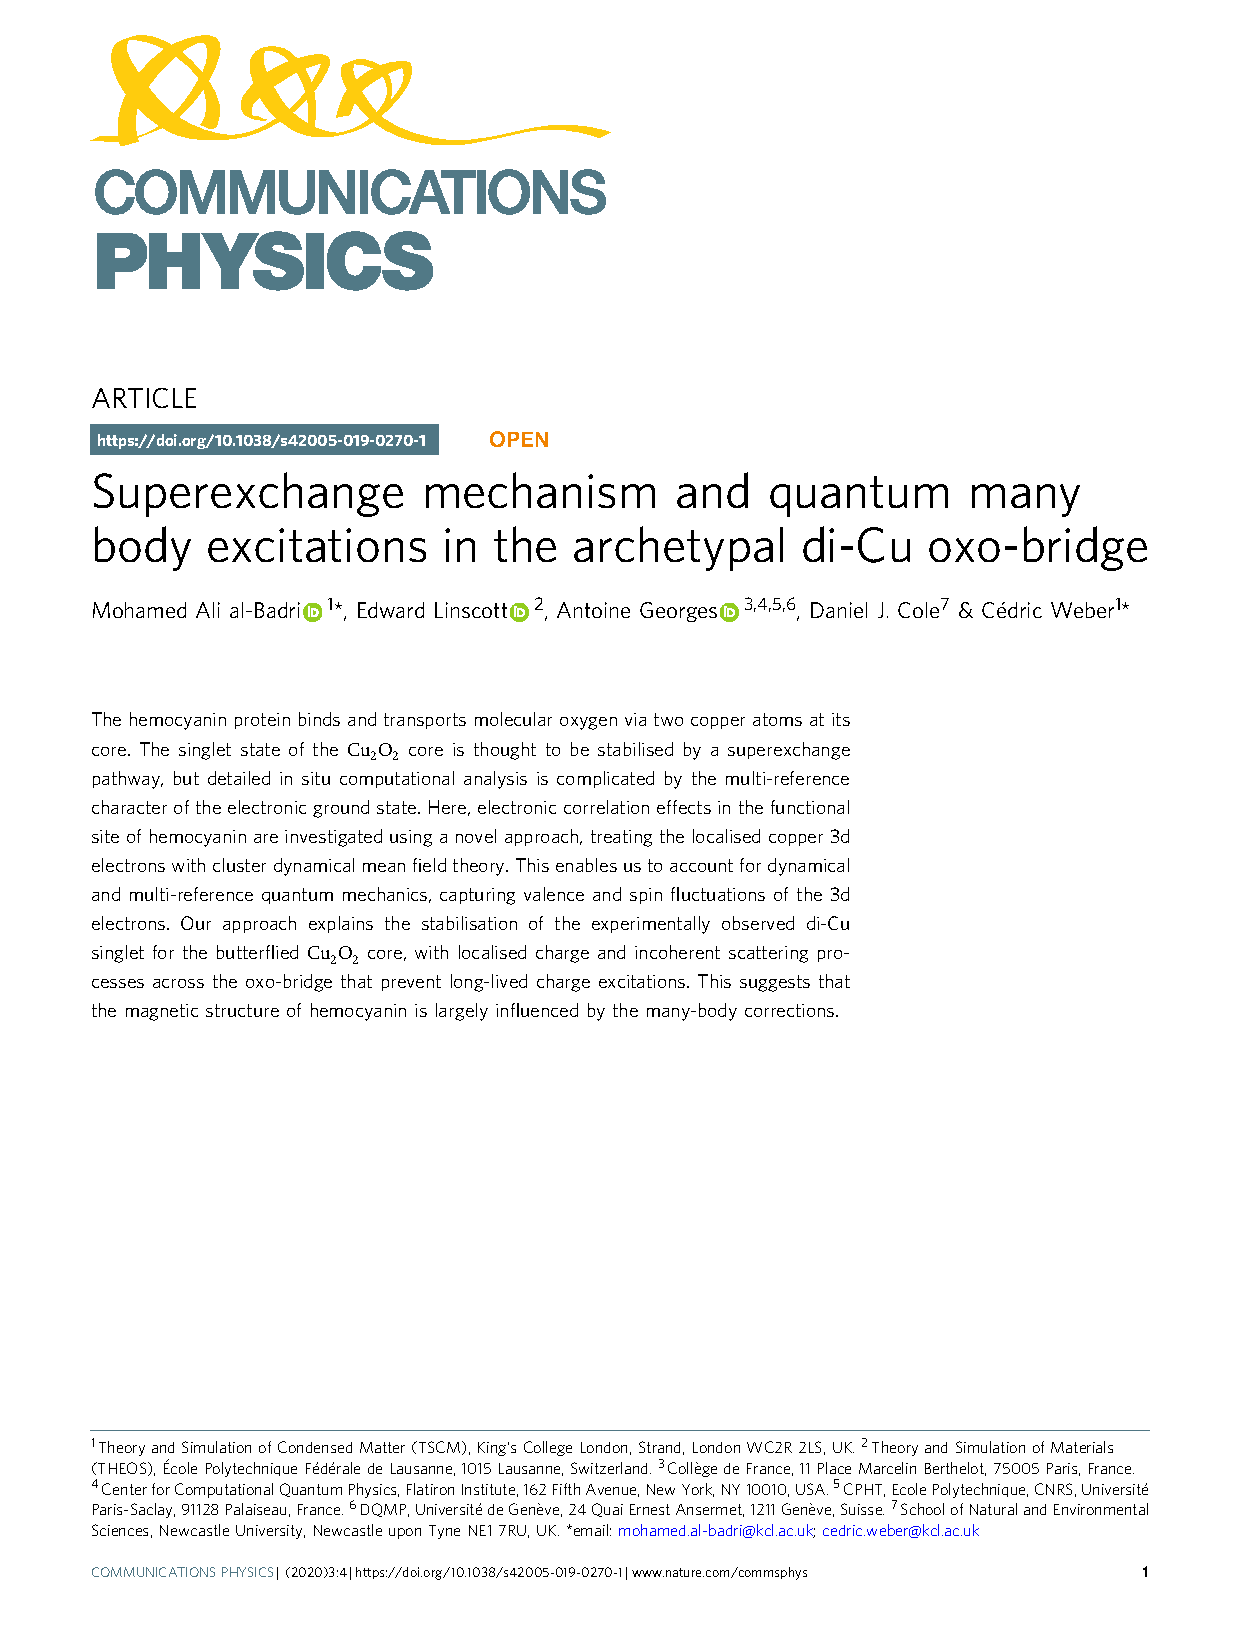
\includepdf[pages=-, offset=75 -75]{PDF_PAPERS/hemocyanin.pdf}


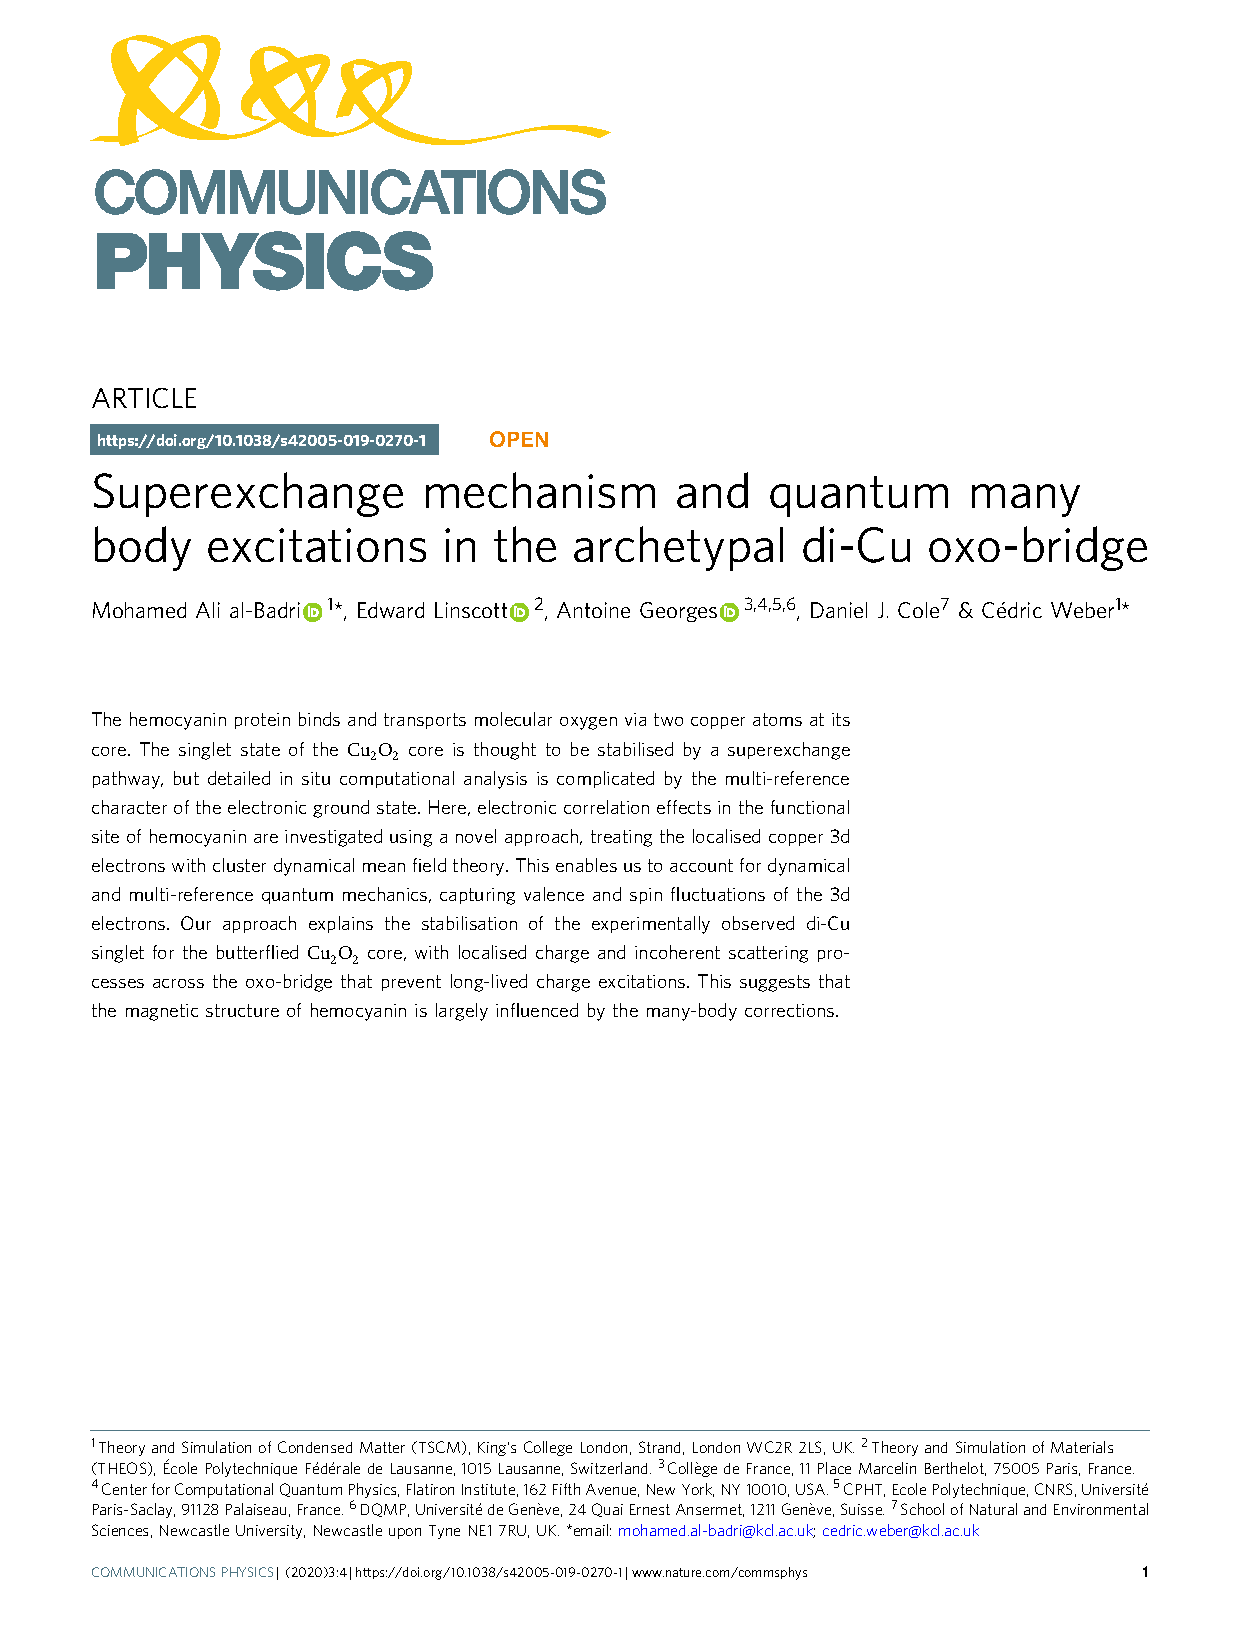
\includepdf[pages=-, offset=75 -75,addtotoc={
     2,section,1,Introduction,pp2,
     2,section,1,Results,pp2,
     2,subsection,2,The spin state of the Cu$_2$O$_2$ core,pp2,
     4,subsection,2,The superexchange mechanism,pp4,
     5,subsection,2,Optical transitions,pp5,
     5,section,1,Discussion,pp5,
     6,section,1,Methods,pp6,
     6,subsection,2,Geometry,pp6,
     6,subsection,2,Density Functional Theory,pp6,
     6,subsection,2,Dynamical Mean Field Theory,pp6},
     addtolist={
     3, figure,{\textbf{The oxyHc functional complex.} Structure showing the Cu$_2$O$_2$ correlated subsystem, which is treated using dynamical mean field theory, and the surrounding imidazole rings representing the protein environment. Hydrogen, carbon, nitrogen, oxygen and iron atoms are shown in white,green, blue, red, and orange respectively.},bb,
     3, figure, {\textbf{The superexchange model of Metz and Solomon.} The Cu$_2$O$_2$ core is depicted from side-on (a,c) and above (b,d). In the planar configuration (a,b), single-ligand orbitals bridge the two copper sites, and superexchange is possible. In a bent configuration (c,d), the copper \textit{d} orbitals overlap with different $\pi^{\ast}$ orbitals. As these two sets of orbitals are orthogonal, hopping between the blue and the red subspaces is not possible and the superexchange mechanism breaks down.},cc,
     4, figure, {\textbf{Decomposition of the reduced density matrix of the Cu$_2$ dimer in the different quantum sectors.} The colours correspond to the respective weights of the different contributions for each value of the Coulomb repulsion $U$ (if a colour occupies all the vertical axis, for example, it means that all eigenvectors of the density matrix are in that particular quantum sector). Note that the $d$ occupation is the sum of both Cu sites (e.g., $d^{20}$ means both Cu atoms are in the $d^{10}$ configuration).},dd,
     4,figure, { \textbf{Dynamical mean field self energy.} a) Imaginary part of the dynamical mean field local self energy $\Sigma(\omega)$ of the Cu-$3d$ empty orbital for Hubbard $U=2$\,eV, $6$\,eV, and $8$\,eV. At $U=8$\,eV, we obtain incoherent excitations at $\omega=0$\,eV. b) The imaginary local self energy at $\omega=0$ and c) the double occupancy of the partially-filled $3d$ orbitals $D$ as a function of $U$. Note that although the double occupancy is evolving smoothly with the Coulomb interaction $U$, $\Sigma(\omega=0)$ shows a sharp increase near $U=8$, associated with the stabilisation of a localised singlet },ee,
     5, figure, { \textbf{Molecular orbital isosurfaces.} The isosurface for the highest occupied molecular orbital (a, c) and lowest unoccupied molecular orbital (b, d) densities for $U = 8$\,eV, as viewed side-on (a, b) and above (c, d). Note that because these are extracted from the Green's function via the spectral density, the phase of the orbitals is inaccessible}, ff,
     5, figure, {\textbf{Theoretical optical absorption of the Cu$_2$O$_2$ core and imidazole rings obtained by dynamical mean field theory for values of the Coulomb repulsion $U=6$ to $10$\,eV.} For comparison, we show the experimental optical absorption in a wide range of wavelengths (infrared to UV). There are several smaller peaks in the experimental spectra that are not visible at this scale (indicated with arrows)}, gg}]{PDF_PAPERS/hemocyanin.pdf}

\includepdf[pages=-, offset=75 -75,addtotoc={
     1,section,1,Supplementary Figures,ppp1,
     4,section,1,Supplementary Notes, ppp4,
     4,subsection,2,Details of diamagnetism, ppp4,
     4,subsection,2,Von Neumann entropy, ppp4,
     5,subsection,2,Natural bond orbital analysis, ppp5,
     6,subsection,2,Atomic coordinates of the model system, ppp6,
     8,subsection,2,Convergence of the system-to-AIM mapping,ppp8,
     8,subsection,2,Local axes, ppp8},
     addtolist={
     1, figure,{The effective magnetic moment $M=\sqrt{\langle \mathbf{S}^2_1 \rangle/3}$  (normalised by saturation value) and the spin correlation $K=2\langle \mathbf{S}_1 \cdot \mathbf{S}_2 \rangle$ for varying values of the Hubbard $U$. For a pure two orbital singlet, $K=-1.5$. In our calculations, as the rest of the molecule hybridises with the Cu orbitals, the spin-correlation is re-normalised to half its saturation value for $U=6-8$\,eV.},aaa,
     1, figure,{The Von Neumann entropy $\Lambda$ of the reduced density matrix and its dependence on the on-site interaction $U$.},bbb,
     2, figure,{Isosurfaces of several natural bonding orbitals for $U = 8$\,eV. (a) Two Cu $3d$ orbitals are identified as half-filled by the NBO analysis. (b) The O\textsubscript{2} $\sigma^*$ anti-bond is empty, and does not hybridise with any Cu orbitals. (c) Instead, O $2p$ (blue) to Cu $4s$ (red) charge transfer is favourable.},ccc,
     2,figure,{(a) The local density of states for $U$ = 8\,eV and (b) the different total density of states of the Cu$_2$O$_2$ functional complex for a range of Hubbard $U$ values from DMFT.},ddd,
     3, figure,{The convergence of the distance $d$ as a function of the total number of sites (impurity and bath).}, eee,
     3, figure,{The local axes for the Cu $3d$ correlated subspaces, and the two half-filled NBOs for comparison.}, fff,
     4, table,{The DMFT $3d$ orbital occupations of Cu in our model of ligated hemocyanin for different Hubbard $U$ values, as calculated using NBO. Note that the orbital labels correspond to the local axes to each Cu atom. All eight other Cu $3d$ orbitals had occupancies $> 1.98$ for all values of $U$}, ggg}]{PDF_PAPERS/SI_hemocyanin.pdf}
%\includepdf[pages=-, offset=75 -75]{PDF_PAPERS/SI_hemocyanin.pdf}




% \chapter{Conclusions}
\label{chapter:conclusions}

%\epigraph{\textit{``Nothing more will I teach you today. Clear your mind of questions.”}}{Yoda}
\epigraph{\textit{I am leaving the regions of fact, which are difficult to penetrate, but which bring in their train rich rewards, and entering the regions of speculation, where many roads lie open, but where a few lead to a definite goal.}}{William Ramsay}


\section{Future work}

%\addcontentsline{toc}{chapter}{Appendices}
\appendix

\chapter{Interpretation of Morphogen Gradients by a Bistable Circuit}
\label{appendix:double-exclusive}
\includepdf[pages=1-51, offset=75 -90, scale=0.85, frame,
        clip,trim=20mm 5mm 20mm 15mm,
        pagecommand={}, addtotoc={
                2,section,1,Supplementary Figures,appendix:double-exclusive:figures,
                18,section,1,Supplementary Methods,appendix:double-exclusive:methods,
                19,subsection,2,Differential Equation Models \& Parameter Inference,appendix:double-exclusive:inference,
                40,subsection,2,Bistability Analysis,appendix:double-exclusive:bistability,
                42,subsection,2,Boundary Experiments,appendix:double-exclusive:boundaries,
                50,subsection,2,Models of the Exclusive Receiver Relay Circuits,appendix:double-exclusive:relay},
        addtolist={
                2, figure, {\textit{Supplementary Figure 1}\quad Circuit variants}, fig:double-exclusive:variants,
                4, figure, {\textit{Supplementary Figure 2}\quad Raw timecourse fluorescence traces}, fig:double-exclusive:plate-data,
                15, figure, {\textit{Supplementary Figure 13}\quad Hysteresis flow cytometry experiments}, fig:double-exclusive:flow-hysteresis,
                41, figure, {\textit{Supplementary Figure 25}\quad Bifurcation curves for uniform and protected degradation models}, fig:double-exclusive:degradation-models,
                41, figure, {\textit{Supplementary Figure 26}\quad ifurcation curve insensitivity specific growth rate $\gamma_0$}, fig:double-exclusive:growth-rate-sensitivity
}]{publications/double-exclusive-si.pdf}

\chapter{Parameter Inference with Bifurcation Diagrams}
\label{appendix:inference}
\includepdf[pages=1-6, offset=75 -90, scale=0.85, frame,
        clip,trim=33mm 20mm 33mm 20mm,
        pagecommand={}, addtotoc={
                1,section,1,Bifurcation Diagrams as Tangent Fields,appendix:tangent-fields,
                2,section,1,Bifurcation Measure Properties,appendix:bifurcation-measure,
                3,section,1,Leibniz Rule for Space Curves,appendix:leibniz-rule,
                5,section,1,Application to the Double Exclusive Model,appendix:more-complex-model,
                6,section,1,Extension for Hopf Bifurcations,appendix:hopf-measure},
        addtolist={
                1, figure, {\textit{Supplementary Figure 1}\quad Two implicit surfaces $f_{\theta}(z)=0$ and $g_{\theta}(z)=0$ in $\mathbb{R}^3$ intersecting to form a space curve which is tangent to field $\tangent(z)$ and perpendicular to gradients $\partial_{z}f_{\theta}$ and $\partial_{z}g_{\theta}$}, fig:implicit-surfaces,
                2, figure, {\textit{Supplementary Figure 2}\quad Left/Right : Determinant $\Det$ and tangent field $\tangent(z)$ for the saddle-node/pitchfork models for some set values of $\theta$ revealing that $\Det=0$ defines bifurcations}, fig:determinant-field,
                5, figure, {\textit{Supplementary Figure 3}\quad Bifurcation inference for the \emph{double exclusive reporter}. A. Optimal parameter estimates $\theta^*$ for the targets $\targets=\{1,2\}$ (indicated by yellow lines in panel B) reveal four regions  with two geometrically different regimes: mutual activation (region 1) and mutual inhibition (regions 2-4). B. Example bifurcation diagrams indicate that region 2 has swapped kinetics between $L$ and $T$ to region 3. Region 4 has models with non-zero imaginary parts to eigenvalues indicating damped oscillations (shown in light green).},
                fig:double-exclusive-optima,
                6, figure, {\textit{Supplementary Figure 4}\quad Bifurcation measure $\measure(s)$ and eigenvalues $\lambda(s)$ along the arclength $s$ for two different bifurcation curves demonstrating how the measure detects non-zero imaginary parts $\Imag[\lambda]$ (onset of damped oscillations marked by circle) and sign changes in real parts $\Real[\lambda]$ (Hopf bifurcations marked by stars)},
                fig:hopf-measure
}]{publications/bifurcation-inference-si.pdf}

\chapter{Exploring Bifurcations between Phenotypes}
\label{appendix:exploring}

\section{Experimental Methods}
\subsection{Tissue Acquisition \& Dissociation} 

All samples were collected via the \href{https://www.cbtm.group.cam.ac.uk}{Cambridge Biorepository for Translational Medicine} under Research Ethics Committee approval 15/EE/0152. Tissue was obtained from five deceased organ donors following circulatory death. Donor metadata is given in Table \ref{table:donors}. Briefly, following cessation of circulatory function donors proceeded to organ donation. Organs were perfused \emph{in situ} with cold organ preservation solution and cooled with topical application of ice. Samples for the study were obtained within 60 minutes of cessation of circulation and placed in University of Wisconsin organ preservation solution for transport at 4°C to the laboratory. Lung and liver samples were obtained from the left lower lobe of the lung and the right lobe of the liver. In addition, two donor-matched blood samples were collected prior to withdrawal of life support, under approval 97/290.

To minimise the possibility of processing-depended differences in cell surface marker expression, all samples, including blood, were processed using enzymatic digestion protocol. Briefly, solid tissues were weighed, transferred into 10cm tissue culture dishes and cut into small pieces. Up to 5g of tissue was then transferred to each of eight GentleMACS C tubes (Miltenyi Biotec) containing 5mL of dissociation media composed of X-vivo15 supplemented with 0.13U/mL Liberase TL (Roche), 10U/mL Benzonase nuclease (Millipore/Merck), 2\% (v/v) heat-inactivated fetal bovine serum (FBS, Gibco), penicillin (100 U/ml, Sigma-Aldrich), streptomycin (0.1 mg/ml, Sigma-Aldrich), and 10mM HEPES (Sigma Aldrich). The samples were then dissociated on a GentleMACS Octo dissociator (Miltenyi Biotec) running a protocol that provided gradual ramping up of homogenisation speed and two 15 minute heating/mixing steps at 37°C. Digested tissue was passed through a 70$\mu$m MACS Smartstrainer (Miltenyi Biotec) and the flow-through was first washed with media supplemented with 2 mM EDTA and then with PBS. Mononuclear cells were enriched by Ficoll-Paque (GE Healthcare) density centrifugation according to manufacturer's instructions. Following, density centrifugation, mononuclear layer was collected, washed once with PBS and cell pellet was resuspended in FACS buffer (PBS, 2.5$\%$ FBS).

Bone marrow aspirates and peripheral blood samples were first subjected to Ficoll-Paque density centrifugation, according to manufacturer's instructions, the mononuclear layer was then collected, washed with PBS and cells were treated with the same dissociation media as solid tissues for 30 min at 37°C prior to washing and resuspension in FACS buffer.

\subsection{Flow Cytometry}

Depending on the cell yield, up to 1x10\textsuperscript{6} mononuclear cells/tissue were stained with antibodies shown in Table \ref{table:panel}. Not all donors were stained with the same panel. To expand total number of markers, sentinel panel design was implemented where CD3 and IgD were detected with antibodies conjugated to BUV395 and Foxp3 and IgM were detected with antibodies conjugated to PE in some donors. Refer to Table \ref{table:panels} for details. 

Single cell suspensions were washed once in PBS, transferred into 96 v-bottom plate and stained with Zombie UV viability dye for 30 min at 4°C following by a wash with FACS buffer. Cell pellets were resuspended in 50$\mu$l FACS buffer with Human FcR block (BD Biosciences) and incubated for 10 min at 4°C. Next, cells were pelleted, excess buffer removed and 100$\mu$l of antibody master mix composed of cell-surface antibody cocktail (see Table \ref{table:panels}), BV buffer (BD) and True-Stain Monocyte Blocker (Biolegend) and incubated for 1h at 4°C. Following incubation, cells were washed three times in PBS and prepared for intracellular staining using transcription factor fixation/permeabilisation kit (eBioscience) according to the manufacturer's instructions. Following IC staining, cell were resuspended in PBS and analysed on BD FACSymphony A3 cell analyser within 10 hours.

\section{Supplementary Tables}

\begin{landscape}
\begin{table}
\footnotesize
\begin{center}
\begin{tabular}{>{\centering\arraybackslash}p{0.6cm}>{\centering\arraybackslash}p{0.4cm}>{\centering\arraybackslash}p{0.7cm}>{\centering\arraybackslash}p{0.9cm}>{\centering\arraybackslash}p{0.9cm}>{\centering\arraybackslash}p{0.9cm}>{\centering\arraybackslash}p{1cm}>{\centering\arraybackslash}p{1cm}>{\centering\arraybackslash}p{1cm}>{\centering\arraybackslash}p{1cm}>{\centering\arraybackslash}p{2.1cm}>{\centering\arraybackslash}p{0.6cm}}
    \toprule
    Donor ID & Sex & Age & Primary cause of death & Multi-trauma & Days in hospital & BMI &CMV/ EBV/ TOXO& Smoking & Alcohol (u/day) & Antibiotics within 2 weeks of death & Steroids \\
    \midrule
    390C & F & 65-70 & ICH & \cmark & 2 & 30-35 & $+$/$+$/$-$ & ? & $<$1 & \xmark & \xmark \\
    403C & M & 50-55 & ICH & \cmark & 8 & 30-35 & $+$/$+$/$-$ & \cmark & $<$1 & Co, T & \xmark \\
    423C & M & 60-65 & ICH & \xmark & 2 & 20-25 & $-$/$+$/$-$ & \cmark & $>$9 & G, F & D \\
    412C & M & 70-75 & ICH & \xmark & 5 & 26-30 & $-$/$+$/$+$ & \cmark & $<$2 & A$^\star$ , F, G, C, Co & P$^\dagger$ \\
    428C & F  & 55-60 & ICH & \xmark & 3 & 20-25 & $-$/$+$/$-$ & \cmark & $>$9 & Co & \xmark \\
    \bottomrule
\multicolumn{12}{p{\linewidth}}{\vline height10pt width0pt
\relax F = Female; M = Male; ICH = intracranial haemorrhage; CMV = Cytomegalovirus; EBV = Epstein-Barr virus; TOXO = Toxoplasmosis; Co = Co-amoxiclav; A = Amoxicillin; T = Tazocin; F = Flucloxacillin; G = Gentamicin; D = Dexamethasone; C = Clarithromycin; \cmark = Yes; \xmark = No; ? = Not known;P = Prednisolone; $^\star$pre-admission, $^\dagger$pre-treatment}\\
\end{tabular}
\caption{Donor Metadata}
\label{table:donors}
\end{center}
\end{table}
\end{landscape}

\begin{table}
\footnotesize
\begin{center}
    \begin{tabular}{llll}
        \toprule
        Specificity & Fluorochrome & Clone & Source \\
        \midrule
        CD3 &  BUV395 & SK7 & BD \\
        CD8 & BUV563 & RPA-T8 & BD \\
        CD69 & BUV737 & FN50 & BD \\
        CD4 & BUV805 & SK3 & BD \\
        CD4 & BUV661 & SK3 & BD \\
        CD45 & BUV805 & HI30 & BD \\
        CD103 & BV421 & Ber-ACT8 & BD \\
        HLA-DR & BV510 & G46-6 & BD \\
        CD127 & PE-Cy7 & HIL-7R-M21 & BD \\
        CCR4 & BV605 & L291H4 & Biolegend \\
        CCR6 & BV650 & 11A9 & BD \\
        PD-1 & BV711 & EH12.1 & BD \\
        CD45RA & BV786 & HI100 & BD \\
        CCR10 & BB515 & 1B5 & BD \\
        CXCR3 & BB700 & 1C6/CXCR3 & BD \\
        CXCR5 & APC-R700 & RF8B2 & BD \\
        CCR7 & APC-Fire750 & G043H7 & Biolegend \\
        CD25 & APC & M-A251 & BD \\
        CD25 & APC & 2A3 & BD \\
        CD19 & BV570 & HIB19 & Biolegend \\
        IgM & PE & G20-127 & BD \\
        IgD & BUV395 & IA6-2 & BD \\
        Foxp3 & PE & 269D/C7 & BD \\
        Foxp3 & PE & PCH101 & eBioscience \\
        Helios & PE-Dazzle & 22F6 & Biolegend \\
        Zombie UV & - & - & Biologend \\
        \bottomrule
    \end{tabular}
\caption{Details of antibodies used in this study}
\label{table:panel}
\end{center}
\end{table}

\begin{table}
\footnotesize
\begin{center}
    \begin{tabular}{lrlll}
        \toprule
        & \multicolumn{4}{c}{Fluorochromes} \\
        \cmidrule{3-5}
         & Panels:&  A &  B &  C \\
        \cmidrule{3-5}
        Specificity & Donor:& 390C & 403C & 412C, 423C, 428C \\
        \midrule
        CD45 && BUV805 & - & - \\
        CD19 && - & - & BV570 \\
        IgM && - & - & PE \\
        IgD && - & - & BUV395 \\
        CD4 && \textbf{BUV661} & \textbf{BV805} & \textbf{BV805} \\
        CD3 &&  BUV395 & BUV395 & BUV395 \\
        CD8 && BUV563 & BUV563 & BUV563 \\
        CD69 && BUV737 & BUV737 & BUV737 \\
        CD103 && BV421 & BV421 & BV421 \\
        HLA-DR && BV510 & BV510 & BV510 \\
        CD127 && PE-Cy7 & PE-Cy7 & PE-Cy7 \\
        CCR4 && BV605 & BV605 & BV605 \\
        CCR6 && BV650 & BV650 & BV650 \\
        PD-1 && BV711 & BV711 & BV711 \\
        CD45RA && BV786 & BV786 & BV786 \\
        CCR10 && BB515 & BB515 & BB515 \\
        CXCR3 && BB700 & BB700 & BB700 \\
        CXCR5 && APC-R700 & APC-R700 & APC-R700 \\
        CCR7 && APC-Fire750 & APC-Fire750 & APC-Fire750 \\
        CD25 && APC & APC & APC \\
        Foxp3 && PE & PE & PE \\
        Helios && PE-Dazzle & PE-Dazzle & PE-Dazzle \\
        Zombie UV && Zombie UV & Zombie UV & Zombie UV \\
        \bottomrule
    \end{tabular}
\caption{Immunophenotyping panel designs used in the dataset}
\label{table:panels}
\end{center}
\end{table} 
% You could separate these out into different files if you have
%  particularly large appendices.

% This line manually adds the Bibliography to the table of contents.
% The fact that \include is the last thing before this ensures that it
% is on a clear page, and adding it like this means that it doesn't
% get a chapter or appendix number.
\addcontentsline{toc}{chapter}{Bibliography}
% Actually generates your bibliography.
\bibliography{biblio}

% All done. \o/
\end{document}
